\documentclass[conference]{IEEEtran}

\IEEEoverridecommandlockouts


\makeatletter
\renewcommand\footnoterule{%
  \kern-3\p@
  \hrule\@width.4\columnwidth
  \kern2.6\p@}
  \makeatother
  
\usepackage{graphicx}
\graphicspath{{fig/}}
\DeclareGraphicsExtensions{.eps,.pdf,.jpeg,.png}

\usepackage[misc]{ifsym}
\usepackage{multirow,booktabs,color,soul,threeparttable}
%\usepackage[ruled,vlined]{algorithm2e}
\usepackage[ruled,linesnumbered]{algorithm2e}
\usepackage{amsmath,bm,setspace}
\interdisplaylinepenalty=2500
\usepackage{amsfonts}
\definecolor{hl}{rgb}{0.75,0.75,0.75}
\sethlcolor{hl}
\usepackage{subfig}
\usepackage{algorithmic}
\usepackage{caption}
\usepackage{afterpage}
\usepackage{array}
\usepackage{stfloats}
\fnbelowfloat
\usepackage{url}
\usepackage{cite}

\newcommand{\semitextbf}[1]{%
	\pdfliteral direct {2 Tr 0.3 w} %the second factor is the boldness
	#1%
	\pdfliteral direct {0 Tr 0 w}%
}

%\def\Plus{\texttt{+}}
\newcommand{\Plus}{\raisebox{.4\height}{\scalebox{.6}{+}}}
% correct bad hyphenation here
\hyphenation{op-tical net-works semi-conduc-tor}

\renewcommand\IEEEkeywordsname{Keywords}

\begin{document}

\title{A New Dynamic Reference Point Specification Mechanism in hypervolume-based EMOA
based on weak convergence detection}

%\author{\IEEEauthorblockN{Linjun He\IEEEauthorrefmark{1},
%Auraham Camacho\IEEEauthorrefmark{2} and
%Hisao Ishibuchi\IEEEauthorrefmark{1}$\textsuperscript{(\Letter)}$}
%\IEEEauthorblockA{\IEEEauthorrefmark{1}School of Electrical and Computer Engineering\\
%Southern University of Science and Technology, Shenzhen, China\\
%Email: helj@mail.sustech.edu.cn, hisao@sustech.edu.cn}
%\and
%\IEEEauthorblockA{\IEEEauthorrefmark{2}CINVESTAV, Tamaulipas, Mexico\\
%Email: acamacho@tamps.cinvestav.mx}}

% use for special paper notices
%\IEEEspecialpapernotice{(Invited Paper)}

\author{\IEEEauthorblockN{Weiduo Liao, Ke Shang, Hisao Ishibuchi} %$\textsuperscript{(\Letter)}$
\IEEEauthorblockA{Department of Computer Science and Engineering\\
Southern University of Science and Technology, Shenzhen, China\\
Email: 11849249@mail.sustech.edu.cn; kshang@foxmail.com; hisao@sustech.edu.cn}
% \and
% \IEEEauthorblockN{Ke Shang}
% \IEEEauthorblockA{Department of Computer Science\\ and Engineering\\
% Southern University of Science\\ and Technology\\ Shenzhen, China\\
% Email: kshang@foxmail.com}
% \and
% \IEEEauthorblockN{Hisao Ishibuchi}
% \IEEEauthorblockA{Department of Computer Science\\ and Engineering\\
% Southern University of Science\\ and Technology\\ Shenzhen, China\\
% Email: hisao@sustech.edu.cn}
}


% make the title area
\maketitle

% As a general rule, do not put math, special symbols or citations
% in the abstract
\begin{abstract}
In the field of indicator-based evolutionary multi-objective optimization algorithms(indicator-based EMOAs), 
hypervolume is a popular indicator, which is the only pareto-compliant indicator up to now. 
But recently, a paper shows that the position of reference point will influence the diversity of the final solutions of
hypervolume-based EMOAs when applying to the inverted-triangular pareto front problems,
by influencing the hypervolume contribution of the external solutions.
In this paper, we state this phenomenon and introduce the reference point adaptation with a dynamic mechanism in terms of necessity.
Then we propose a new dynamic mechanism based on weak convergence detection. 
In our approach, the simple Least Squares and the information of nadir point are used to detect the convergence. 
After that, we examine the difference between this new dynamic mechanism with a state-of-the-art linearly decrease mechanism. 
\end{abstract}

\begin{IEEEkeywords}
reference point adaptation; indicator-based algorithm; hypervolume; evolutionary multi-objective optimization; 
behavior; dynamic mechanism; convergence detection
\end{IEEEkeywords}
    
\let\thefootnote\relax\footnotetext{This work was supported by the Program for Guangdong Introducing Innovative and Entrepreneurial Teams (Grant No. 2017ZT07X386), Shenzhen Peacock Plan (Grant No. KQTD2016112514355531), the Science and Technology Innovation Committee Foundation of Shenzhen (Grant No. ZDSYS201703031748284), the Program for University Key Laboratory of Guangdong Province (Grant No. 2017KSYS008), and National Natural Science Foundation of China (Grant No. 61876075).}

% For peer review papers, you can put extra information on the cover
% page as needed:
% \ifCLASSOPTIONpeerreview
% \begin{center} \bfseries EDICS Category: 3-BBND \end{center}
% \fi
%
% For perreview papers, this IEEEtran command inserts a page break and
% creates the second title. It will be ignored for other modes.
\IEEEpeerreviewmaketitle

% -------------------------------------- main part ---------------------------------------
% 背景介绍:
% 在indicator based 算法里,HV作为唯一的compliant indicator被广泛使用
% SMSEMOA是最简单的一种indicator based 算法   μ+1机制
% FVEMOA是SMSEMOA的一种优化 速度更快 用了 μ+m机制
% reference point要slightly larger then 1+1/H at beginning then decrease to 1+1/H,  
% hisao的paper with linearly decrease mechanism: 
% [1] H. Ishibuchi, R. Imada, N. Masuyama and Y. Nojima. 
% Dynamic Specification of a Reference Point for Hypervolume Calculation in SMS-EMOA[J].
% Proc. of 2018 IEEE Congress on Evolutionary Computation (IEEE CEC 2018)
% 介绍我的 new mechanism:weak convergence detection decrease
% 一篇paper介绍一种robust and efficient的convergence detection criterion
% Introducing a Robust and Efficient Stopping Criterion for MOEAs
% 但是对象是针对indicator的,而我们的算法运行中计算的indicator 
% 每一代的evaluation不一样,没有可比性
% 补充一张记录每次evaluation时以当时estimated的reference point为based 的hv值的图,
% 表示没有可比性(用FVEMOA的)
% 于是我想到了用nadir point的mean来当indicator,表示是否接近pareto front
% 实验图 mean of ln(nadir point)和它的bsf 与hv的变化曲线基本一致
%(hv斜率变0的时候 这个新indicator的斜率也差不多变成0)
% 介绍一个windows 和 windows内的简单线性回归。 
% 因为会有恶化和停滞现象 所以window size要设置的大一点,
% 经过实验用4000次evaluation作为window size不错
% 然后画b的图,给出经过实验 threshold选10^-5不错。
% 实验
% 4种problems要一句话介绍
% 
\section{Introduction}
In the field of evolutionary multi-objective optimization algorithms (EMOAs), 
several researchers focus on various indicators including hypervolume\cite{hypervolume}, R2\cite{R2}, $\epsilon_+$ indicator\cite{e+} and IGD\cite{IGD}.
The indicators are designed for different purposes, and as a matter of fact, 
have their own strong points and drawbacks. Different from IGD, 
hypervolume does not need the pre-knowledge of the shape of the pareto front 
and is the only pareto-compliant indicator up to now\cite{pareto_compliant}. 
But with a heavy computation load of hypervolume computation\cite{hypervolume:computationLoad}, 
the hypervolume-based algorithms get poor performances 
in running time when dealing with problems which have more than three objectives, 
which is so-called Many-Objective Optimization Problems(MaOPs). 

In order to reduce the heavy computation cost of hypervolume computation, 
many new indicators or new methods have been proposed to estimate the hypervolume. 
For example, HypE use a Monte Carlo simulation technology to estimate the effect of hypervolume\cite{HypE}; 
R2 indicator bases on a standard weighted Tchebycheff function\cite{R2} and a new R2 is proposed by Shang et al\cite{newR2}.
Recently, an improved SMS-EMOA with adaptive resource allocation has been proposed to reduce the number of hypervolume calculations\cite{ismsemoa}; 
In 2015, a simple and fast version of SMS-EMOA\cite{smsemoa}, so-called FV-EMOA, has been proposed\cite{FVEMOA}.
In order to further reduce the bottleneck of high time complexity for calculating the hypervolume contributions, 
the FV-EMOA considers the fact that the hypervolume contribution of a single solution 
is only associated with partial solutions rather than the whole solution set\cite{FVEMOA}. 
Based on this point, the FV-MOEA reduces the computational cost greatly. 
In this paper, the FV-MOEA is used in the experiment section, 
for its better performance on time-saving than SMS-EMOA\cite{FVEMOA}. 

The specification of the reference point is one of the important parts in hypervolume computation. 
It has been reported that the position of reference point strongly influences the value of
hypervolume contribution of the external solutions on the problems with inverted-shape pareto fronts\cite{hisao:RPhowtoSpecify, hisao:RPspecify, hisao:RPexplanation}. 
A suitable set of reference point position for flat pareto fronts has been sufficiently investigated in Hisao st al\cite{hisao:RPspecify}.
And a dynamic reference point adaptation has also been proposed in Hisao st al\cite{hisao:dynamic}.
Another strategy proposed is to use two reference points in hypervolume-based EMOA\cite{hisao:twoRP}. 
In this paper, the dynamic mechanism is stated in two different stages of the algorithm running process. 
At the early stage, for a better searching behavior of the algorithm, 
the reference point should be set a little worse than the suggested position at the beginning.
Then by a dynamic mechanism, the reference point is gradually decreasing to the suggested position following the iteration. 

After that, we propose a new dynamic reference point adaptation with a weak convergence detection in hypervolume-based EMOA. 
The simple least squares and the logarithm value of nadir point as a convergence indicator are used in this weak convergence detection. 
For a given window $w_l$ generations, if the slope of linear regression is below one threshold, we report the convergence.
The comparison of two dynamic mechanisms and simple reference point adaptation(without dynamic mechanism) is 
discussed in the experiment section. On some specific conditions, for example, when the total evaluation number 
is limited to a small addition after the reported convergence, our weak convergence detection mechanism 
outperforms the linearly decrease mechanism. 

The remainder of this paper is organized as follows. 
Firstly, we briefly introduce the basic idea of reference point adaptation by a simple example in Section II.
Then, we state the reference point adaptation with the dynamic mechanism in Section III.
The necessity of a dynamic mechanism is also illustrated in this Section. After that,
the details of the new dynamic mechanism proposed in this paper is in Section IV. 
And we report our computational experiments of FV-EMOA
with several triangular and inverted-triangular problems in Section V. our experiments are performed on
3- and 5-dimension problems for clearly comparing of two dynamic mechanisms and 
simple reference point adaptation (without dynamic mechanism). Finally, the conclusion is shown in Section VI.

% --------------------------- reference point specification in hypervolume-based EMOA ---------------------
% reference point不应该只在刚开始设置而后面都不变,这样如果问题的feasible region很大的时候,初始设置的
% reference point就会离PF很远(画图一个很大的feasible region和PF和reference point)
% 这样的话 在某些问题(倒三角)最后分布在PF上的解 边缘上的解分布很密集【hisao paper】【倒三角图,r很大】
% 因此 necessity of a good reference point specification during the progress of algorithm
%
% 在很多算法中 include SMSEMOA
% The reference point is specified by the following common-use role:
% estimated reference point = r × estimated nadir point, r = 1.1, 
% the estimated nadir point is the vector consists of every maximization objective values of all
% solutions in current population.【图】
%
\section{Reference Point Specification in Hypervolume-based EMOA}
When hypervolume(HV) is used in indicator-based algorithms, 
one important thing to be considered is how to specify the reference point.
Before calculating the HV values, a reference point needs to be chosen in advance.
However, it is not suggested that the reference point is set only once at the beginning. 
This may cause a very far away reference point from solutions
for those problems with a very large feasible space(As shown in Fig. \ref{rpa1}),
as the solutions set is gradually converging to the pareto front
during the iteration of the algorithm process.

\begin{figure}[!t]
  \centering
  \subfloat[The initial generation.]{\label{rpa1:a}
    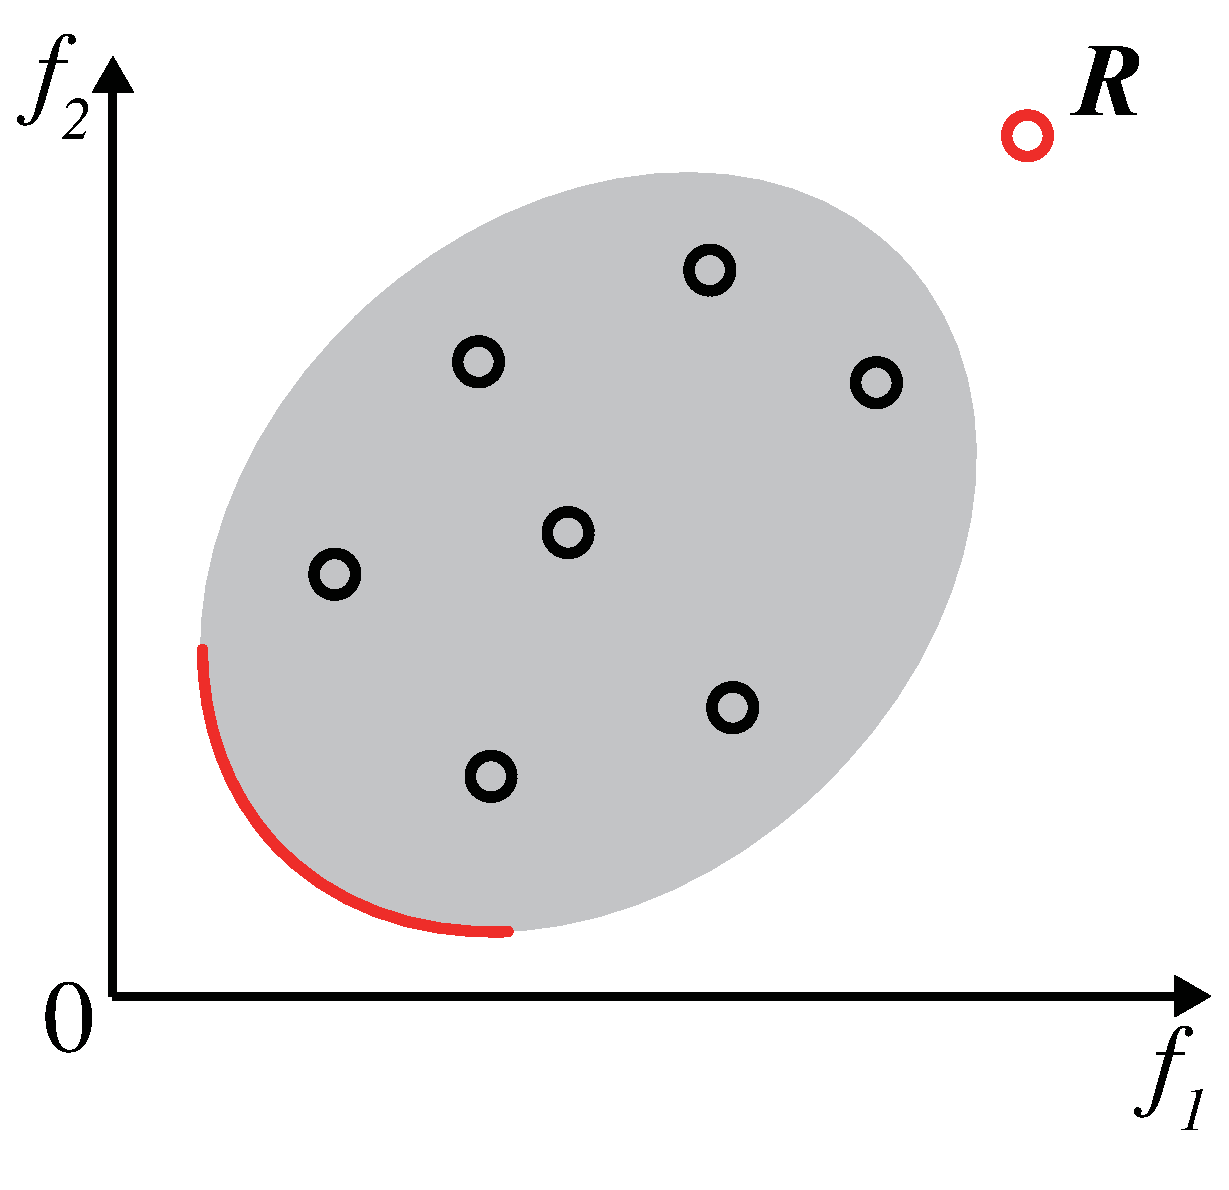
\includegraphics[width=1.5in]{rpa1_1}}\quad
  \subfloat[The final generation.]{\label{rpa1:b}
  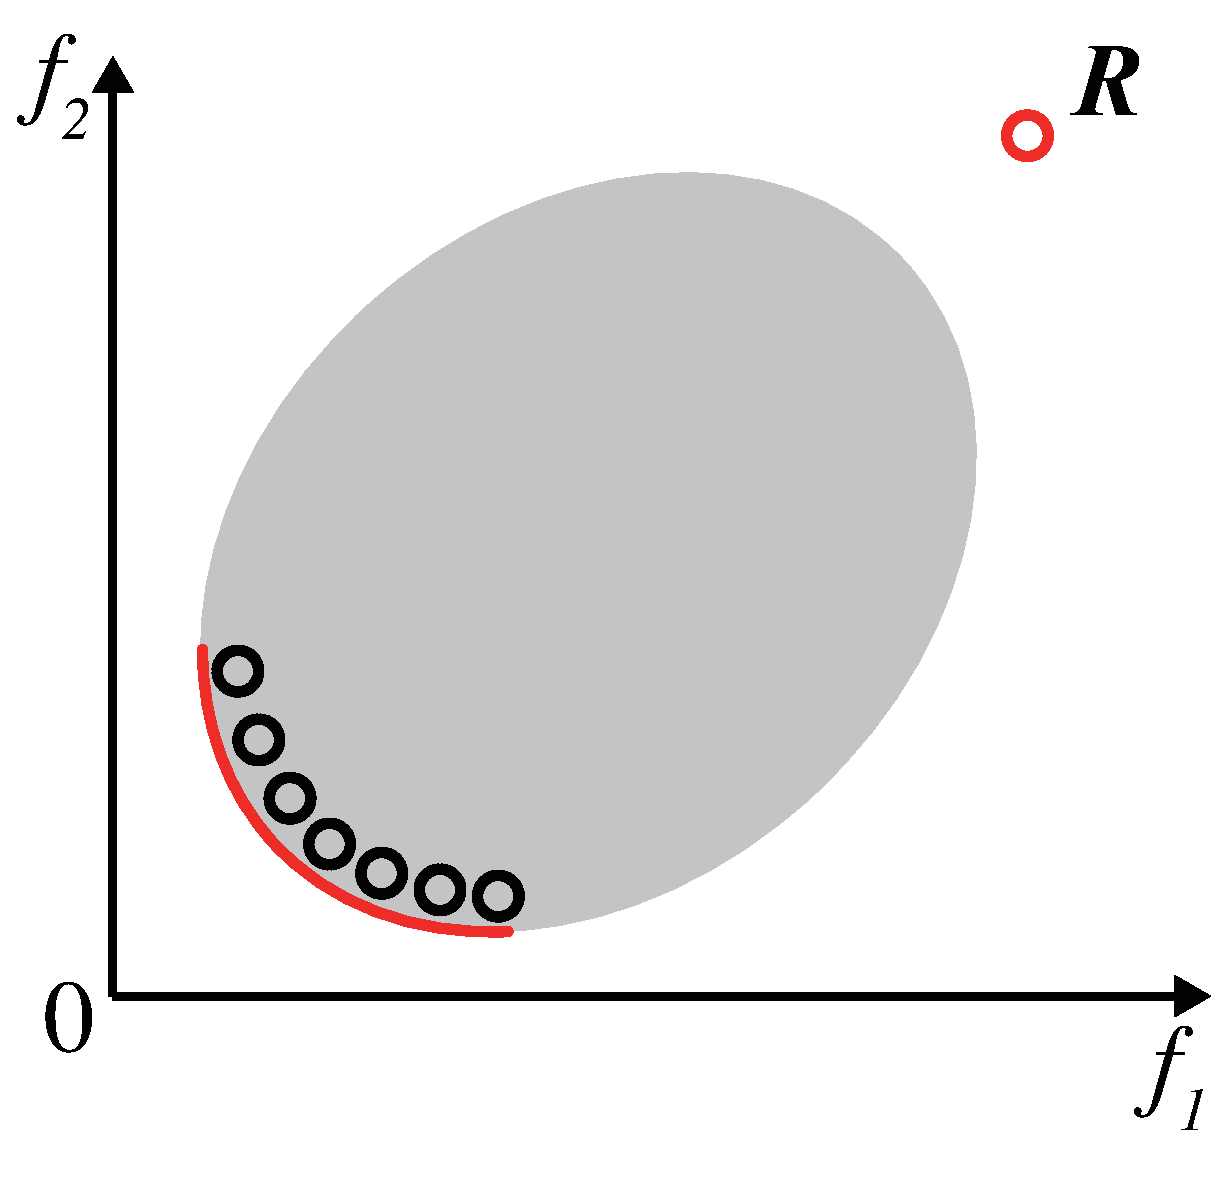
\includegraphics[width=1.5in]{rpa1_2}}\\
  \caption{The reference point is set with a large feasible space.
  pareto front can be far away from reference point.
  The gray region shows the feasible region and the red arc is the corresponding pareto front.
  The red circle $r$ is the reference point calculated by the initial solutions in (\ref{rpa1:a})
  which is randomly generated.
  After some generations, the current solutions reach to the five black circles in (\ref{rpa1:b}), 
  which is far away from the reference point.}
  \label{rpa1}
\end{figure}

There is a big problem when applying this strategy to some problems with specific pareto front shape, 
for example, the inverted-DTLZ1 problem with an inverted-triangular pareto front in 3 dimensions,
that many solutions in the final solutions set will distribute at the boundary of the pareto front
(Fig. \ref{rpa2:a} comparing with Fig. \ref{rpa2:b})\cite{hisao:RPexplanation, hisao:RPspecify, hisao:dynamic}. 
Although it has no effect on the distributions of solutions set 
in problems with triangular pareto front in 3 dimensions 
(Fig. \ref{rpa2:c} comparing with Fig. \ref{rpa2:d}), 
it is necessary using a good reference point specification method during the algorithm progress.
And the reason is illustrated detailedly in Hisao et al\cite{hisao:RPexplanation}.

\begin{figure}[!t]
  \centering
  \subfloat[The reference point is fixed.]{\label{rpa2:a}
    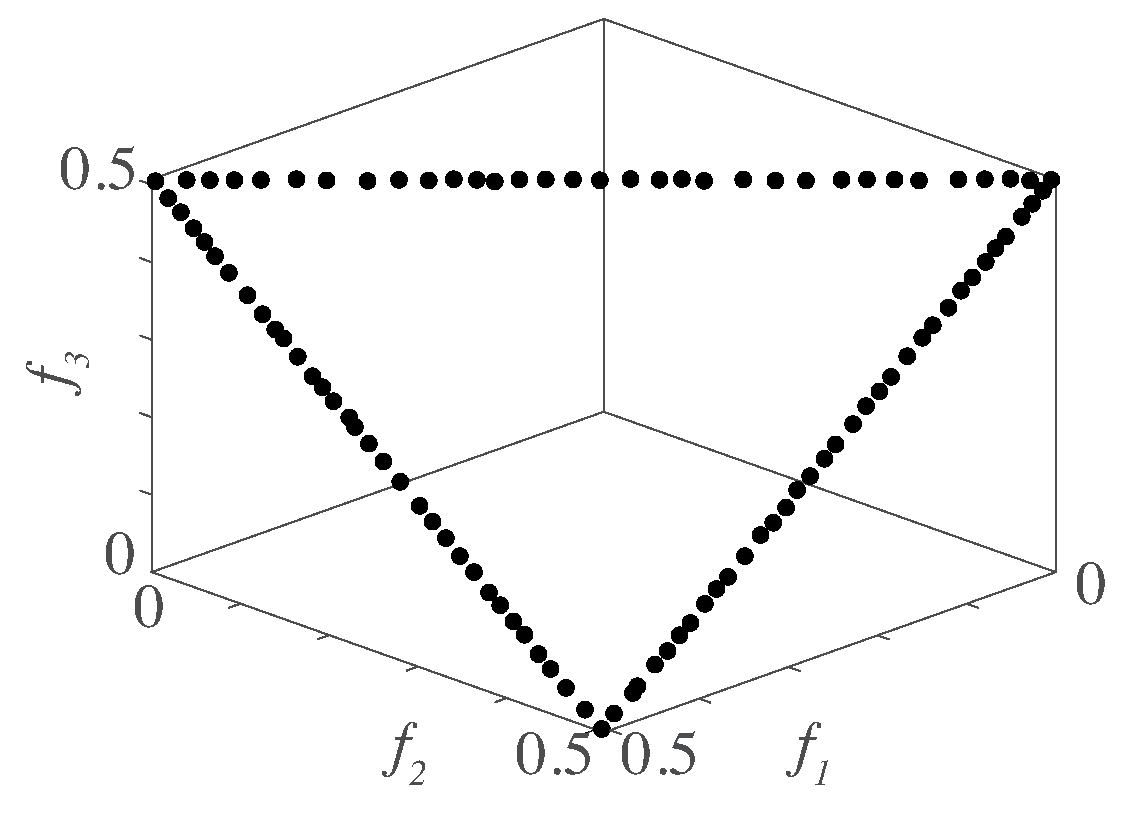
\includegraphics[width=1.5in]{FVEMOA_fixrp_IDTLZ1_evaluation20000_r1__1}}\quad
  \subfloat[The reference point is specified by the formula (\ref{frpa1}).]{\label{rpa2:b}
    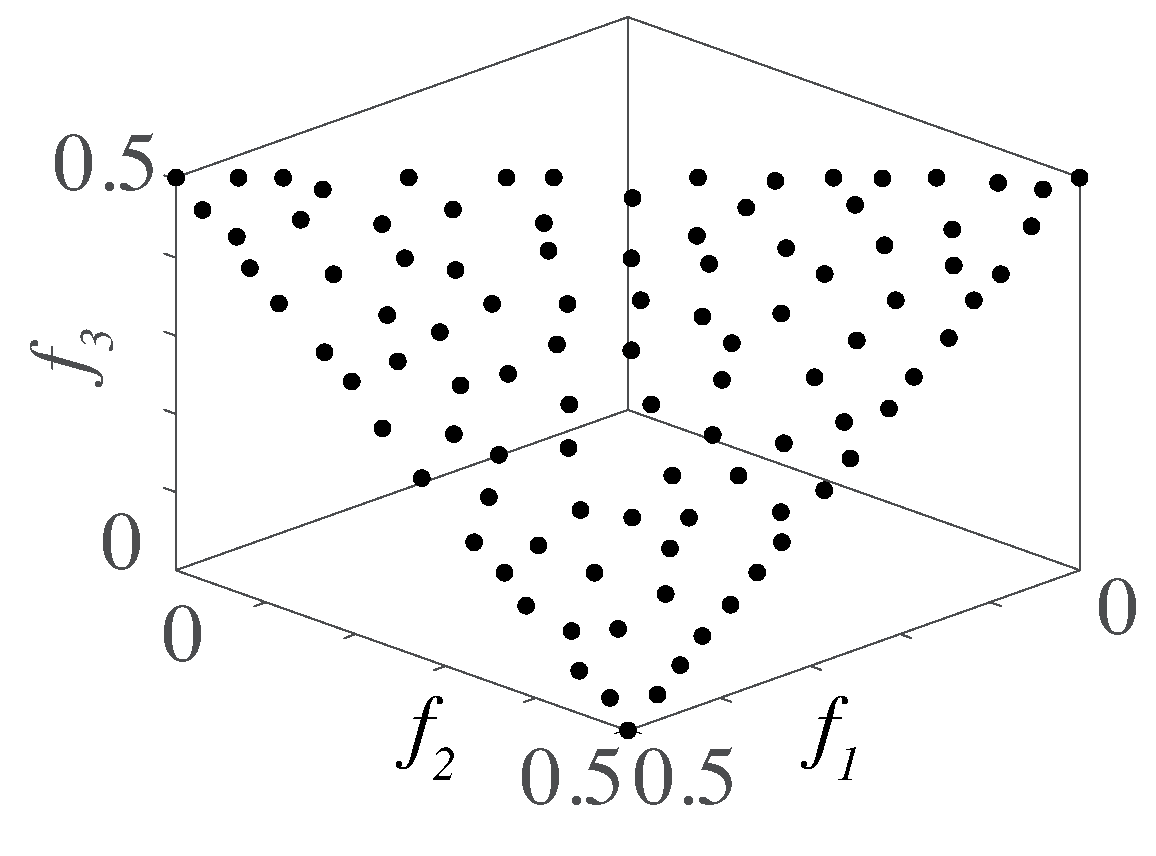
\includegraphics[width=1.5in]{FVEMOA_IDTLZ1_evaluation20000_r1__1}}\\
  \subfloat[The reference point is fixed.]{\label{rpa2:c}
    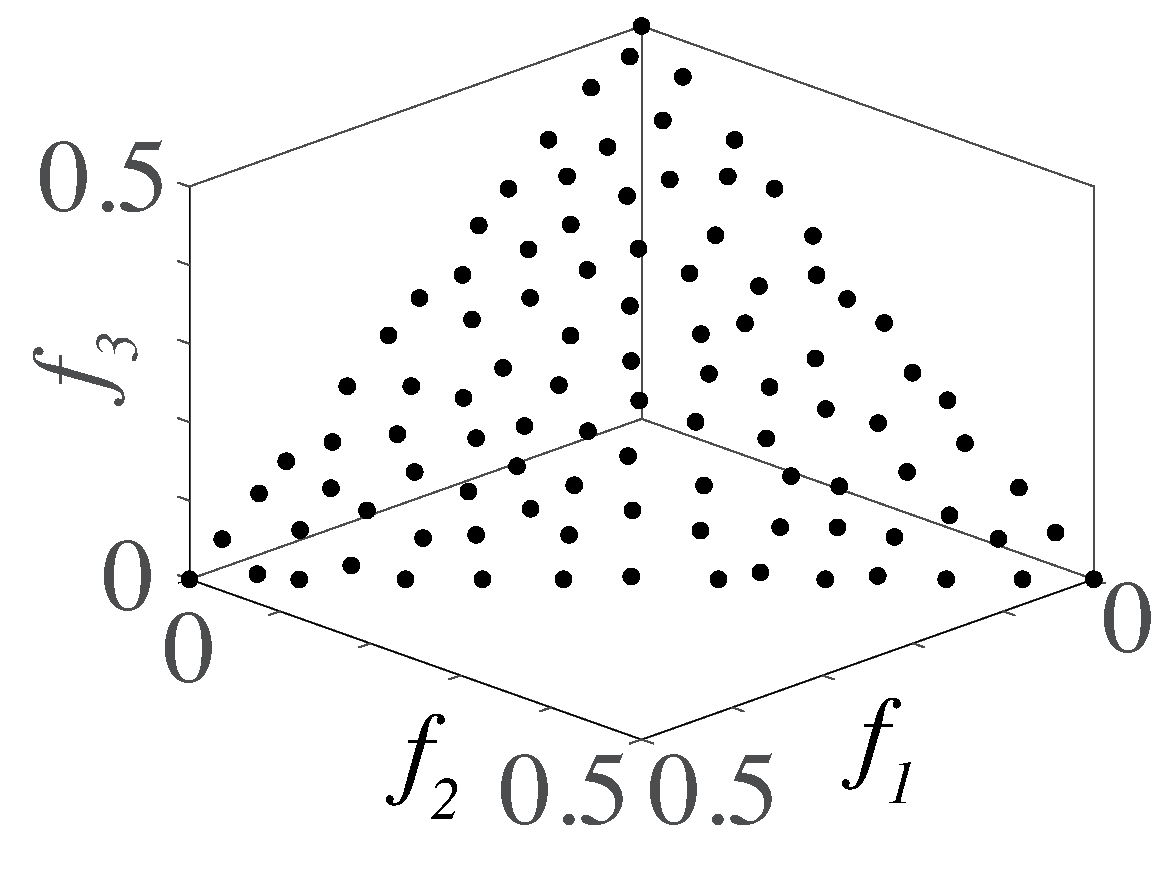
\includegraphics[width=1.5in]{FVEMOA_fixrp_DTLZ1_evaluation20000_r1__1}}\quad
  \subfloat[The reference point is specified by the formula (\ref{frpa1}).]{\label{rpa2:d}
    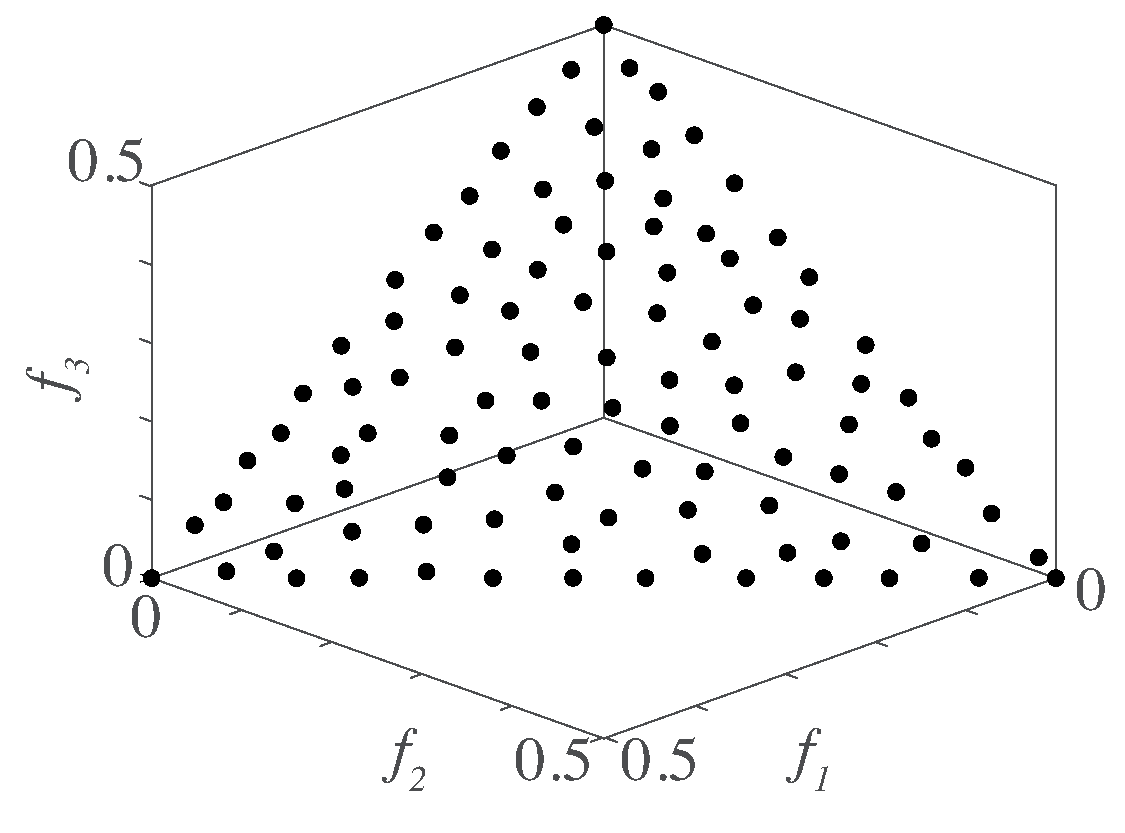
\includegraphics[width=1.5in]{FVEMOA_DTLZ1_evaluation20000_r1__1}}\\
  \caption{The final distribution of solutions set in the inverted-DTLZ1(\ref{rpa2:a} and \ref{rpa2:b}) 
  and the DTLZ1 problem(\ref{rpa2:c} and \ref{rpa2:d}).
  The algorithm is FV-EMOA with population size $= 100$, evaluation number $= 20000$ and $r=1.1$. 
  (\ref{rpa2:a} and \ref{rpa2:c}): the reference point is calculated only once at the initial step;
  (\ref{rpa2:b} and \ref{rpa2:d}): the reference point is specified by the formula (\ref{frpa1}).
  All the solutions in the final distribution are at the boundary of the pareto front in (\ref{rpa2:a}),
  which shows the bad effect of a faraway reference point
  on the final distribution of inverted-triangular problems.
  This bad effect can not be observed on triangular problems in (\ref{rpa2:c}).
  }
  \label{rpa2}
\end{figure}

In many algorithms including SMS-EMOA\cite{smsemoa}, 
the reference point is specified based on the following rules:
\begin{equation}\label{frpa1}
  RP = r * ENP, r = 1.1.
\end{equation}
Note that the estimated nadir point($ENP$) is the nadir point in current population.
When the solutions in the current population are obtained, 
we use hypervolume as the indicator to evaluate the performance of the solutions set. 
Then the reference point used to calculate the hypervolume is calculated by the formula above.
%可以加一个介绍nadir point的图,如果8页不够的话。 !!!!!!!!

% ----------------------------------- dynamic mechanism ------------------------------------
% 在算法运行的不同时期 early stage;final stage, 为了不同的目的,
% (early stage是convergence, final stage是diversity) r应该设置成不同的值【我的本科毕设和hisao】
% 即 r value 应该是随着算法的进行dynamically设置成不同的值。 
%
% unfortunately 对r的研究太少了, 因为在 benchmark问题上, 特别是正三角 r对PF上的解的影响很小
% 但是实际上 在一些问题上 最后PF上解的分布情况是对r很敏感的【hisao paper里的倒三角和最近点问题】
% 
\section{the Dynamic Reference Point Specification Mechanism}
However, the suggested value of $r$ is investigated in \cite{hisao:RPexplanation, hisao:RPhowtoSpecify, hisao:RPspecify}.
$r=1.1$ is not a suggested value, especially on problems with a flat(not concave or convex) pareto front.
Based on the formula (\ref{frpa1}), 
we define the dynamic reference point specification as that,
 a adaptive value of $r$ during the process of algorithm.

Basically, the process of Evolutionary Multi-objective Optimization Algorithm can be separated into
two stages:
\subsubsection{Early Stage} In this stage, 
all the solutions are far away from pareto front.
The main task is to converge the solutions to pareto front.
We also call this stage the convergence stage.
\subsubsection{Final Stage} In this stage,
all the solutions are in or near the pareto front.
So the main task is to make the distribution of solutions more evenly in the pareto front.
We also call this stage the diversity stage.

For different purposes in these two stages, the $r$ should be treated differently\cite{hisao:dynamic}. 
Not only the reference point but also the value of $r$ 
needs to be adapted in each iteration of the algorithm. 
This is called dynamical reference point adaptation. 

Unfortunately, the research on how to specified $r$ is limited.
Only a few papers\cite{hisao:RPexplanation, hisao:RPhowtoSpecify, hisao:RPspecify} 
did some research on the optimal setting of the reference point on 
flat (not concave or convex) pareto front problems. 
The reason is that the effect of the location of the reference point on the pareto front 
is not fatal on some benchmark problems, especially triangular pareto front. 
But in fact, on some specific problems, the distribution of solutions on pareto front
strongly depends on the location of the reference point. 
The sensitivity about the value of $r$ for solutions is also observed on some real-world problems,
for example, distance minimization problems.
This observation potential shows the usefulness of the dynamical reference point adaptation
\cite{hisao:dynamic}.

In this section, we will specify the suggested $r$ values separately
in the early and final stages.

% ------------------sub-------------- reference point specification in hypervolume-based EMOA ----------------------------------
% --------------- reference point specification for optimal distribution ----------------
% 在hisao的paper中指出r = 1+1/H 在一些问题中(平的PF问题)是最优的设置(画出二维三维图for example),
% 提一句 本文主要的研究问题就是平的PF问题
% 即在算法的最后final stage,所有solution都在PF上,r应该设置成1+1/H。
%
\subsection{Specify the Value of $r$ for Optimal Distribution}
In the final stages, the major purpose is to augment the diversity of solutions set.
More specifically, for inverted-triangular problems, in order to have same hypervolume contribution, 
the interval between two boundary solutions should be the same as that between two inner solutions.
In hisao st al\cite{hisao:RPhowtoSpecify}, the suggested value of $r$ for flat(not concave or convex) pareto front problems is:
\begin{equation}\label{eod}
  r=1+\frac{1}{H},
\end{equation}
as shown in Fig. \ref{dm1}. $H$ is the number of solutions intervals in 2-dimension 
and the number of interval at each boundary of pareto front in many-dimension.
In Fig. \ref{dm1:a}, $r=1.2(H=5)$ is the optimal setting for a $21$ individuals 
inverted-DTLZ1 problem and a evenly distribution is observed. 
In Fig. \ref{dm1:b} - Fig. \ref{dm1:d}, the inner solutions are decreased and move to
the boundary of pareto front. 

\begin{figure}[!t]
  \centering
  \subfloat[$r=1.2$(optimal).]{\label{dm1:a}
    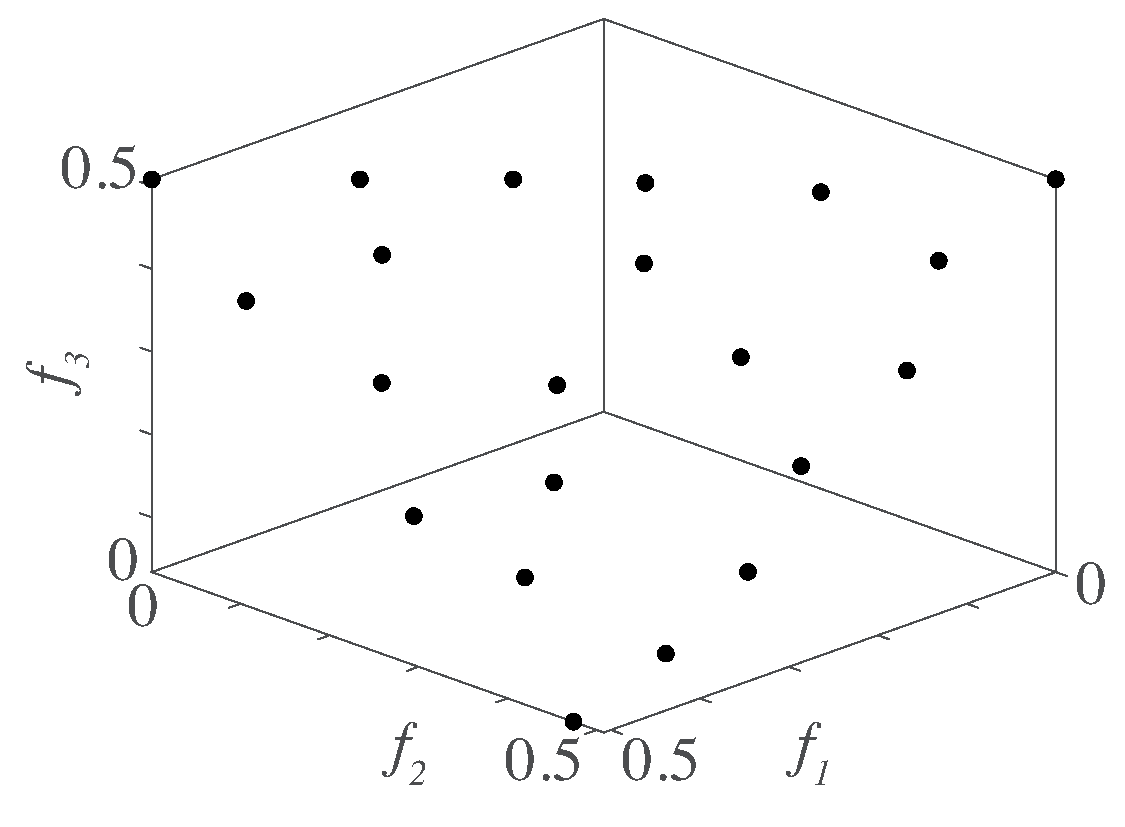
\includegraphics[width=1.5in]{FVEMOA_IDTLZ1_evaluation10000_r1__2_N21}}\quad
  \subfloat[$r=1.5.$]{\label{dm1:b}
    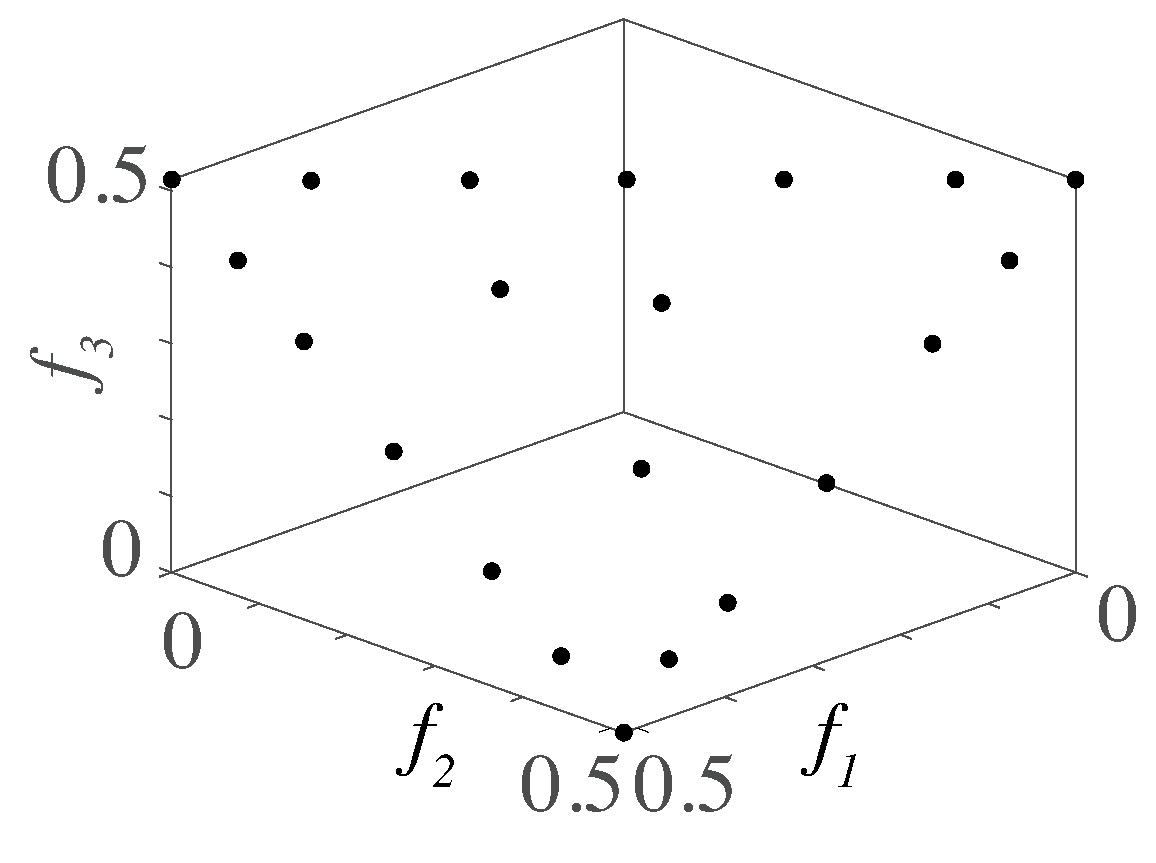
\includegraphics[width=1.5in]{FVEMOA_IDTLZ1_evaluation10000_r1__5_N21}}\\
  \subfloat[$r=2.$]{\label{dm1:c}
    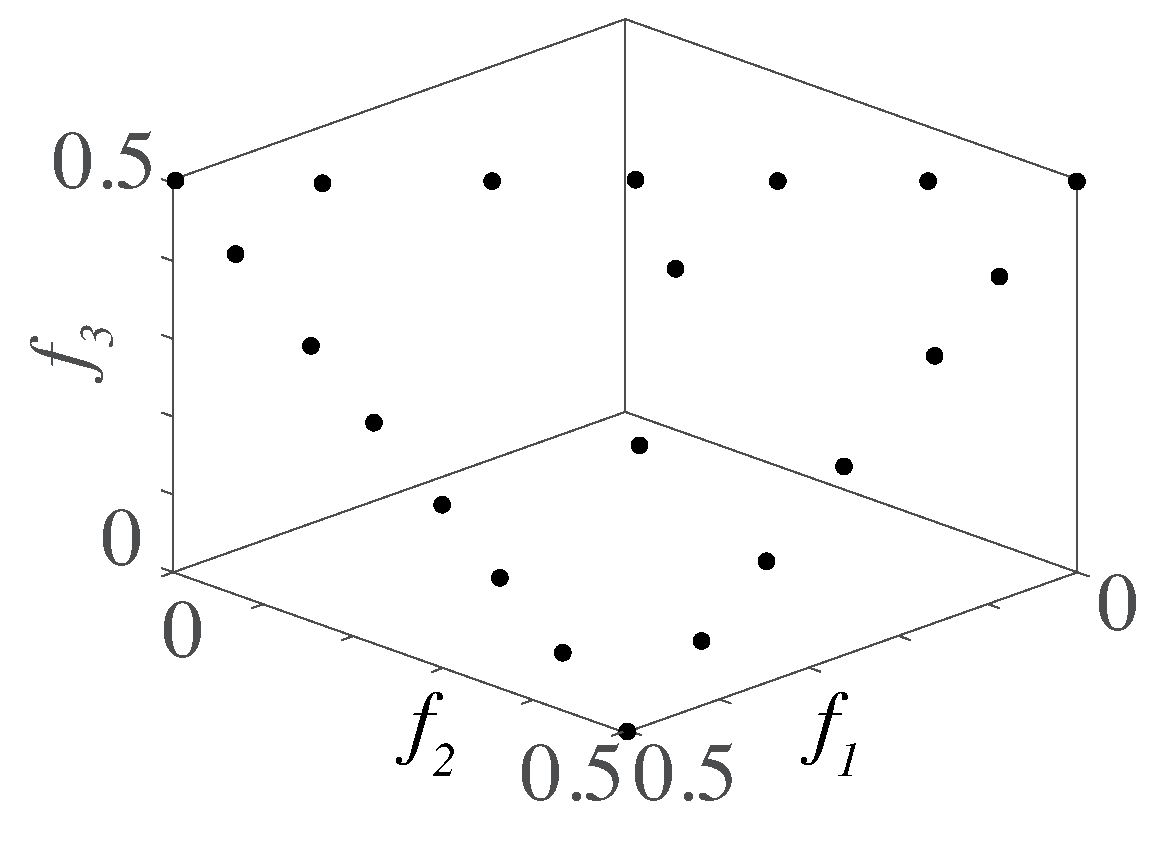
\includegraphics[width=1.5in]{FVEMOA_IDTLZ1_evaluation10000_r2_N21}}\quad
  \subfloat[$r=5.$]{\label{dm1:d}
    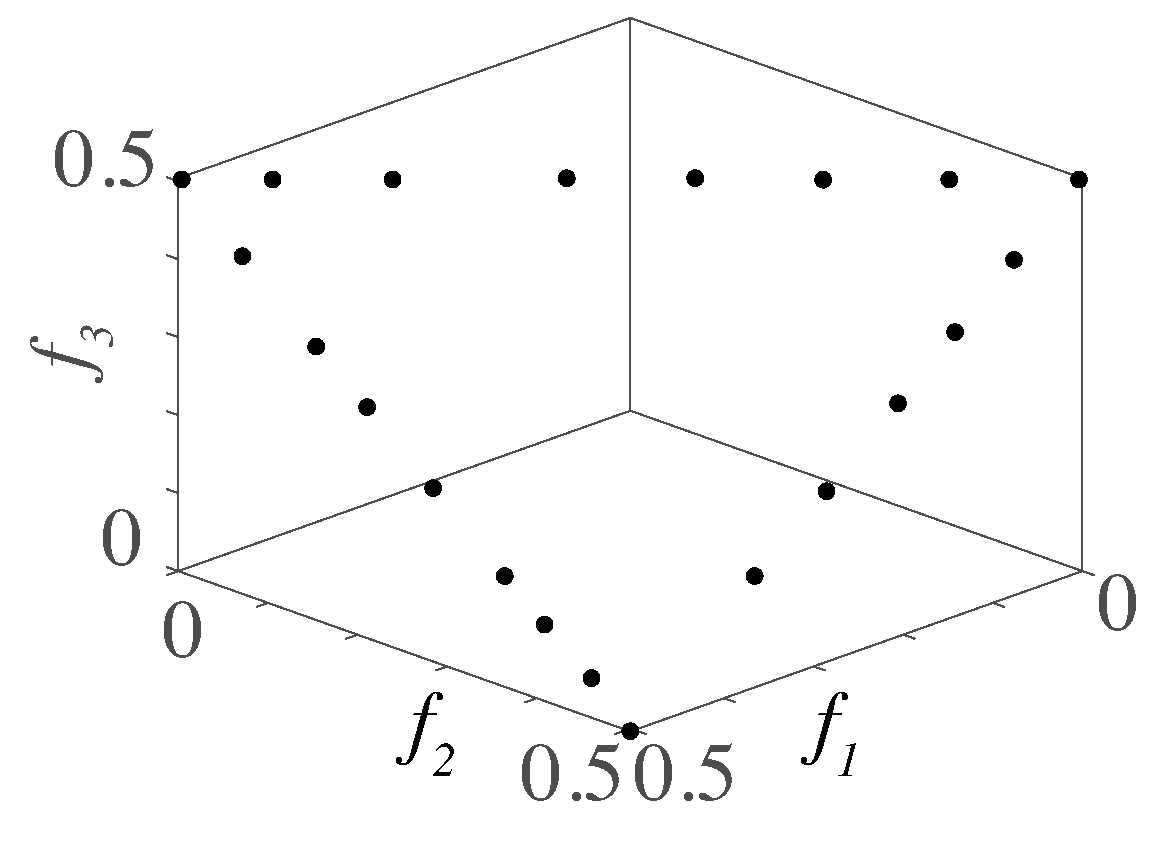
\includegraphics[width=1.5in]{FVEMOA_IDTLZ1_evaluation10000_r5_N21}}\\
  \caption{The final distribution of solutions set in the inverted-DTLZ1 problem.
  The algorithm is FV-EMOA with population size $=21$($H=5$) and evaluation number $=20000$.
  $r=1.2$ is the optimal setting and we observed a evenly distribution in (\ref{dm1:a}).
  As the increasing of $r$, solutions are more likely to be at the boundary
  (\ref{dm1:b}-\ref{dm1:d}). 
  }
  \label{dm1}
\end{figure}

For simple illustration,
when algorithm reaches to the final stage, all solutions are near the pareto front, $r$ should
be specified as $1+1/H$, as in equation \ref{eod}. 

% ------------------sub-------------- dynamic mechanism ----------------------------------
% --------------- reference point specification for better searching behavior ------------
% hisao指出如果一直用1+1/H, 在convergence阶段会有不好的 search behavior,因为
% specify 1+1/H in each generation, 在 early generations
% the estimated ideal and nadir points from the nondominated
% solutions in each generation 离PF太远。
% 因此 对于normalization based on the estimated ideal and nadir points 
% often has unexpected bad effects on the search behavior
%
% in early generations, a slightly larger r is suggested in 【hisao和我的本科毕设】
% 大一点的r能够加快convergence 用NHV试试 log(HV)
% (加图 相同的evaluation 一直optimal和一直2 一直2会快点收敛 一个HV 一个NHV, 
% HV表示最后hv差,NHV表示较快到达前沿)
% (图 r越大,收敛越快,从三维开始 画出hv变化斜率图)
% 
\subsection{Specifiy the Value of $r$ for Better Searching Behavior}
However, in the early stage, solutions set is not close to the pareto front, which makes the 
estimated ideal and nadir points far away from true ideal and nadir points, for the reason that
they are calculated by current solutions in each generation. 
And considering some problems without an easy mapping from decision space to objective space,
if the external solutions have the same hypervolume contribution with the inner solutions,
the exploration of pareto front will be poor. 
As a result, the solutions can hardly jump out from the local minimums and the diversity will be poor.
Two examples are given in the experiment section (As shown in Fig. \ref{iudm1:d} and \ref{iudm2:d}). 

In \cite{hisao:dynamic}, a larger value of $r$ than the $1+1/H$ is suggested in the early stage.

% ------------------sub-------------- dynamic mechanism ----------------------------------
% ------------------------- linearly decrease mechanism --------------------------
% so r从2到1+1/H 很必要 之前介绍过 但是怎么变化 没有一个特别好的idea outperform the others
% hisao的paper,提到一种linearly decrease 机制 就是从2到1+1/H线性下降 这是一种简单又实用的idea
% 图在下一个section画。
% 接下来本文介绍一种基于weak convergence detection criterion, 在一些限制条件下outperform线性机制。
% 
\section{Linearly Decrease Mechanism}
Based on the theory above, $r$ is suggested to be specified dynamically at different stages of
the algorithm(at early stage, a slightly larger $r$ is chosen; at final stage, $r=1+1/H$ is chosen).
But unfortunately, there is no best mechanism on how to specify the value of $r$ dynamically
outperforms the others in all problems and all experiment settings. One mechanism may be the best
when working on some specific experiment conditions, but may not be good on other conditions. 

In \cite{hisao:dynamic}, a linearly decrease mechanism has been proposed:
\begin{equation}\label{eldm1}
  r(t)=r_{Initial}\frac{(T-t)}{T}+(1+1/H)\frac{t}{T}, t=0,1,\dots,T,
\end{equation}
where $T$ is the total number of generations, and $r_{Initial}$ is the initial value of $r$,
which is larger than $1+1/H$.
It is a simple and practical mechanism. In (\ref{eldm1}), the value of $r$ starts from $r_{Initial}$,
then gradually decreases to the suggested value in a linearly decrease process. 

In the next section, we will propose another good dynamic mechanism based on weak convergence 
detection criterion outperforms simple linearly decrease mechanism on some constraint condition.

% -------------------------------- new dynamic mechanism ------------------------------------
% 本文介绍一种基于weak convergence detection criterion的 new mechanism
% 当 检测到convergence 就把r从2变成optimal 
% (画 r 随 evaluation变化图 就是z字型那个 和线性机制一起画)
% 
\section{New Dynamic Mechanism}
In this section,
we will introduce a new mechanism that uses a weak convergence detection criterion to 
decide whether to change the value of $r$ from $r_{Initial}$ to $1+1/H$. 

As we have explained before, 
a slightly larger $r$ is suggested at the initial stage of the algorithms. 
But for good diversity at the final stage,
it is needed to set $r$ to its optimal value ($1+1/H$). 
For this purpose, we detect whether the algorithm is converged or not.  
If solutions are all close to the pareto front, 
we change the value of $r$ to $r_{Optimal}$; otherwise, we set value of $r$ to 
$r_{Initial}$. The mechanism is also shown below:
\begin{equation}\begin{aligned}\label{endm1}
  r(t)&=r_{Initial}\mathbb{I}\left[t<t_{Convergent}\right]\\
  &+(1+1/H)\mathbb{I}\left[t \ge t_{Convergent}\right], t=0,1,\dots,T,
\end{aligned}
\end{equation}
where $\mathbb{I}$ is the indicator function returning $1$ if argument is true and $0$ otherwise.
$r(t)$ equals to $r_{Initial}$ before reaching to the convergent generation $t_{Convergent}$,
and changes to $1+1/H$ after $t_{Convergent}$. 
The $t_{Convergent}$ is determined by a weak convergence detection criterion. 

% ---------------sub-------------- new dynamic mechanism ------------------------------------
% ----------------------------- weak convergence detection ----------------------------------
% consider some convergence detection paper【各种 convergence detection paper】
% convergence detection一般用各种各样的indicator【各种paper】
% 总结特点:用indicator list的太花时间;精确的收敛检测
%
% 准则:
% convergence detection 不应该花太多时间,并不需要太准  用 subsubsection
% 需要寻找一种不需要花太多计算量的 weak criterion
% 【一些paper】indicator based algorithm用indicator
% for us,it seems to be a good idea to use HV 作为indicator,however
% 但是程序运行过程中 hv的reference point 一直在变,所以不同generations没有可比性
% (画一张算法运行过程中用的hv的图)
%
% estimated nadir point 会越来越接近PF, 并且当solutions reach to PF后 NaidrP stagnation
% (画 HV和bsf ln(nadir point) mean的图 最好用MaF1的 可能平滑些)表示它们同时期变化。 
% good idea to use ln(nadir point) mean作为判断解是否reach to PF 的 indicator
% 一篇论文(Introducing a Robust and Efficient Stopping Criterion for MOEAs)实现了
% the Least Squares Stopping Criterion for convergence detection 
% when indicator has reached a stagnation situation, stop
% 用一种简单并且直观SIMPLE INTUITIVE 的方式 就是剩余价值和线性回归斜率 below thresholds
% 介绍机制 线性计算公式
% 画上图(ln np mean)的b随evaluation变化图
% for nadir point, 经过我们的实验 10^-5是个好threshold
%
\subsection{Weak Convergence Detection}
Consider many convergence detection papers 
\cite{convergenceDetection:1, convergenceDetection:LSSC, convergenceDetection:OCD, 
convergenceDetection:OFCDandOCD, convergenceDetection:convergenceMetric, convergenceDetection:maxCD, 
convergenceDetection:online},
various indicators including convergence detection indicators are using to detect the stagnation.
They focus on the accuracy of convergence, which is not the purpose in our approach for 
the reason that after algorithm convergent, we still need some generations in order to
get even distribution of solutions set. 
We summarize our weak convergence detection criterions as follow:
\subsubsection{inaccuracy} It is no need to have an accurate convergence detection. 
The convergence can be reported if current solutions are close to the pareto front.
In other words, the estimated ideal and nadir points based on the current solutions
are close to the true ideal and nadir points. 
\subsubsection{saving time} We should not spend too much time in convergence detection
for the reason that the state-of-the-art indicator-based algorithms such as SMS-EMOA and HypE, 
are time-consuming when the dimension is very high. 

We are discussing the effect of reference points in calculating hypervolume. It seems to be a good
idea to use progress indicator hypervolume as our convergence detection indicator, 
for that, we have calculated 
hypervolume in each generation in the hypervolume-based evolutionary multi-objective optimization algorithm.
But during the process of algorithm, the reference point is calculated by (\ref{frpa1}) 
in each generation.
So we can not just simply compare hypervolume calculated in algorithm among different generations. 

We are trying on some other good indicators satisfying our convergence detection criterions. 
Fig. \ref{wcd1} shows the change of hypervolume(HV) and nadir point on the FV-EMOA algorithm 
with the 3-dimensional inverted-DTLZ1 problem.
When current solutions are close to the pareto front, the estimated nadir point is close 
to the true nadir points. 
\begin{figure}[!t]
  \centering
    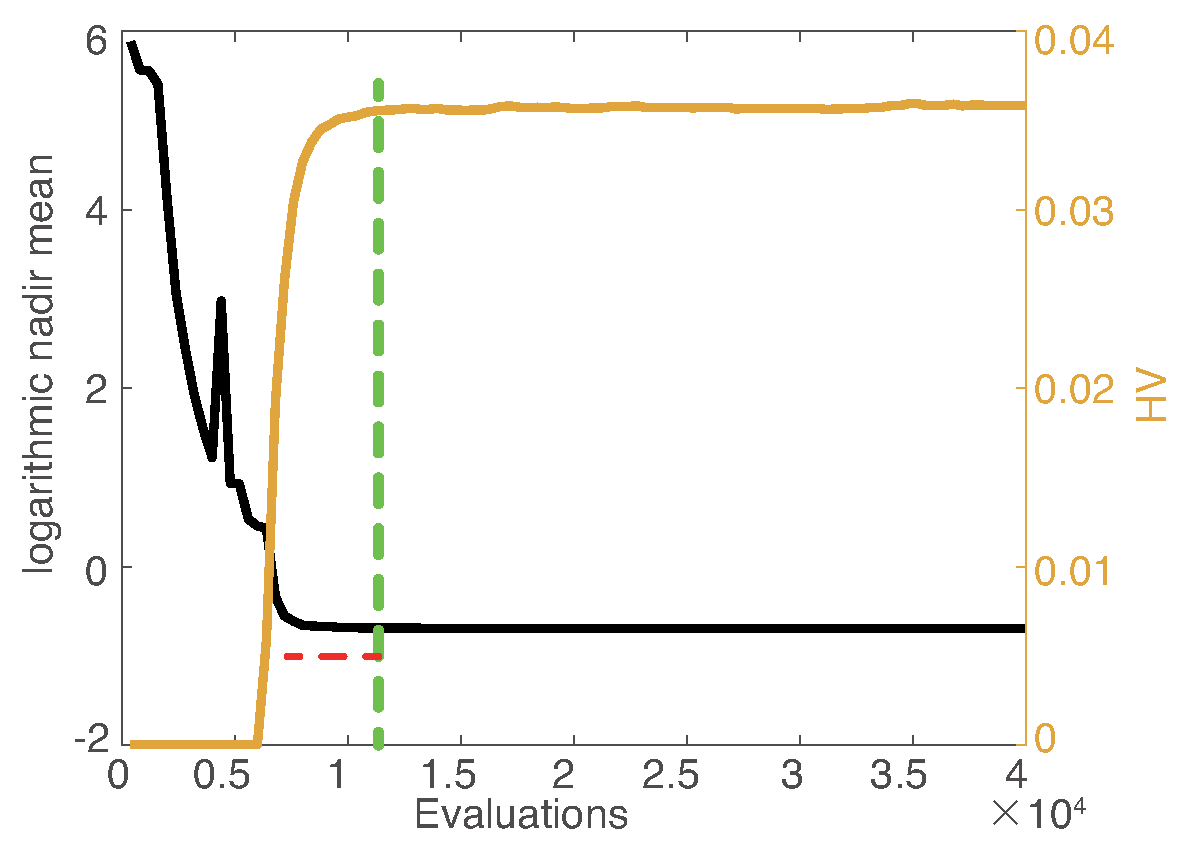
\includegraphics[width=\columnwidth]{FVEMOA_IDTLZ1_M3_nadir_1}
  \caption{Example of nadir point and hypervolume(HV) value on inverted-DTLZ1 3-dimension problem
  with FV-EMOA algorithm.
  The yellow curve is the change of hypervolume 
  while the black curve is the change of logarithmic nadir point.
  }
  \label{wcd1}
\end{figure}
This implies that the estimated nadir point can be a good indicator of our purpose. 
But for some problems with the large feasible region, 
the moving distance of the estimated nadir point in the early generations is larger than that near convergence.
So we consider the logarithm. And considering the possible bad variance of the indicator, 
finally, we use the best logarithmic nadir point so-far as our indicator. more specifically,
for a minimization problem, we consider the indicator as follows:
\begin{equation}\begin{aligned}\label{ewcd1}
  ENP_{t} &= [f_{t1},f_{t2},\dots,f_{tm}]^\top \in \mathbb{R}^m ,\\
  I_{0} &= \frac{1}{m} \sum_{i=1}^{m}lnf_{0i},\\
  I_{t} &= min(I_{t-1},\frac{1}{m} \sum_{i=1}^{m}lnf_{ti}),
  t = 1,2,\dots,T,
\end{aligned}
\end{equation}
where $T$ is the total number of generations, 
$ENP_{t}$ is the estimated nadir point at the $t$th generation with $m$ objectives $f_{t1},f_{t2},\dots,f_{tm}$. 
$I_0$ is the initial indicator calculated by the initial population.
And $I_t$ is the minimum value before the $t$th generation (including the $t$th generation). 

After chosen the indicator, the next step is to detect the stagnation of the indicator.
We use a basic linear regression method called Simple Least Squares\cite{SimpleLeastSquares} with a
simple least squares convergence detection strategy introduced in \cite{convergenceDetection:LSSC}.
If the absolute value of the slope of the indicator is below a threshold, the convergence is reported.
Briefly speaking, for a simple linear regression $I=a+bt$,
the intercept $a$ and slope $b$ of the $t$th generation can be calculated 
with the following matrix-based formula:
\begin{equation}\label{elr1}
  \left[
    \begin{matrix}
      a \\
      b
    \end{matrix}
  \right]
  = 
  \left[
    \begin{matrix}
      \sum t_i^2 & \sum t_i \\
      \sum t_i   & w\_ l 
    \end{matrix}
  \right]^{-1}
  *
  \left[
    \begin{matrix}
      \sum t_i * I_{t_i} \\
      \sum I_{t_i} 
    \end{matrix}
  \right]
\end{equation}
where $w\_ l$ is the length of the chosen window 
and $t_i$ is the evaluated number in the chosen window.
The value of slope $b$ is shown in Fig. \ref{wcd2} 
(Note that the value in the first $w\_ l$ evaluations is 0, 
and we should not consider the first $w\_ l$ evaluations). 
\begin{figure}[!t]
  \centering
    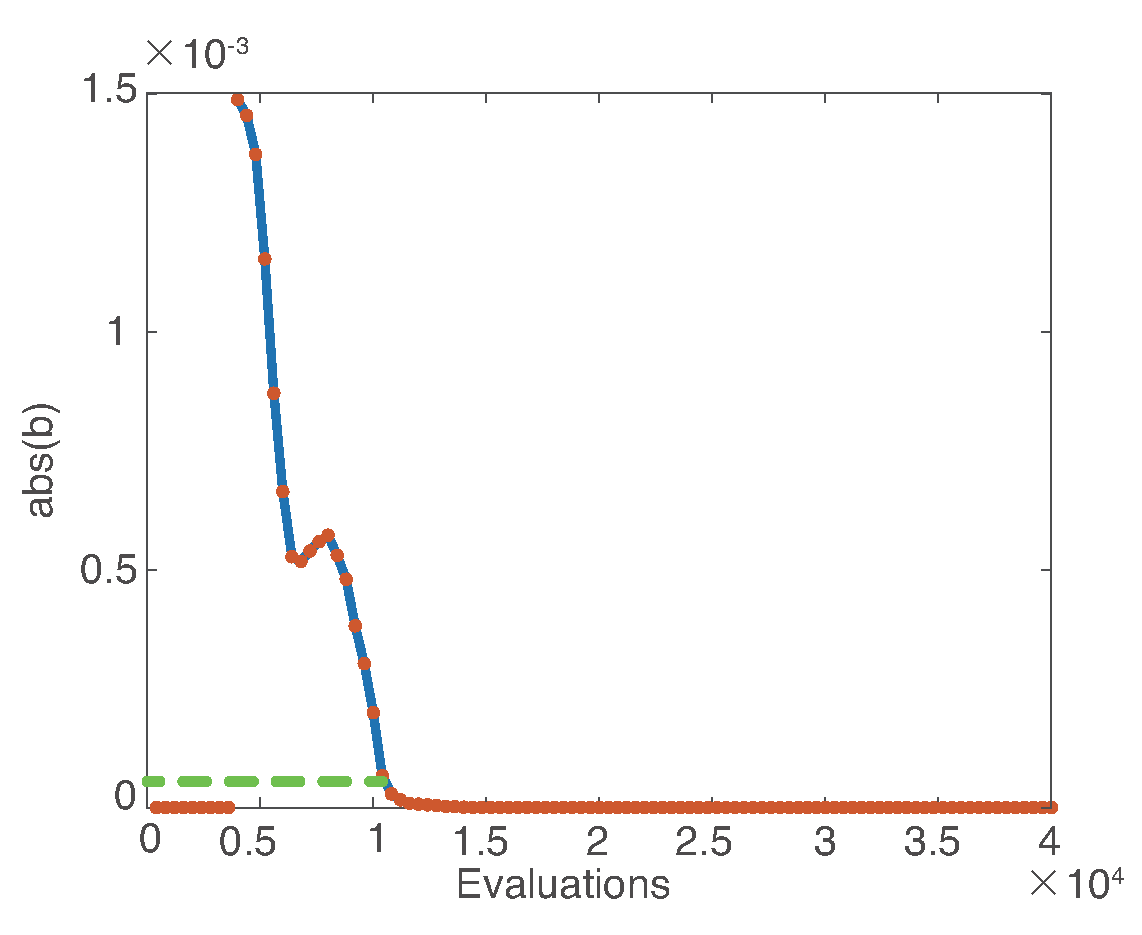
\includegraphics[width=\columnwidth]{FVEMOA_IDTLZ1_M3_nadir_2}
  \caption{Example of $\lvert b\rvert$ on inverted-DTLZ1 3-dimension problem
  (window size = $4000$ evaluations with population size = $100$).
  }
  \label{wcd2}
\end{figure}

With the above formula (\ref{elr1}), the convergence detection criterion is defined as:
\begin{equation}\label{elr2}
  convergence = \lvert b \rvert < thres
\end{equation}
The chosen of the $thres$ value is not so important 
as the report ahead or delay is not fatal to the algorithm or to the final solutions set.
We choose the $thres$ value as $10^{-5}$ after some experimental computation with 
the window size $w\_ l = 4000$ evaluations. 
If we do not change the window size, 
this threshold can be applied to other problems or indicator-based algorithms
because of a weak convergence detection purpose.

% -------------------------------- Computational Experiments ------------------------------------
% 为了直观的表现dynamic reference point adaptation的优势,
% 算法 sets 我们选用了什么,简单介绍
% 我们选用了test problem:DTLZ1, C1_DTLZ1,IDTLZ1,MaF1 分别介绍
% 维度选择了 3,5,8,10维 为了表现在multi 和 many上的不同
% 
% compare this mechanism with the linearly decrease mechanism
% 
% 要验证 10^-5 是不是一个好的threshold 画出不同维度 当检测到收敛的solutions图,确认检测到不变的时候确实收敛
%
\section{Computational Experiments}
To clearly represent the superiority of dynamically reference point adaptation 
and to ease the comparison process of two different dynamic mechanisms
(linearly decrease mechanism and weak convergence detection mechanism), 
the mechanisms are going to be tested with the algorithm FV-EMOA\cite{FVEMOA}.
The problems include: 
DTLZ series\cite{DTLZ}, WFG series\cite{WFG} and their minus versions\cite{minusTestProblem}
and two inverted-triangular pareto front problems: 
Inverted-DTLZ1\cite{hisao:RPexplanation}, MaF1\cite{MaF}.
To show the performance both on multi-objective and many-objective, we tested in 3 and 5 dimensions.
All the code in this section is implemented in PlatEMO framework\cite{PlatEMO} 
with the following additional settings:

Population size: 100, 

Total evaluation number: 400,000 solution evaluations,

Crossover: simulated binary (probability: 1.0),

Mutation: polynormal (probability: $1/n$),

Number of decision variables $n$:

$\qquad m+4$ (DTLZ1, minus-DTLZ1, inverted-DTLZ1),

$\qquad m+9$ (other problems),

Distribution index in Crossover and Mutation: 20, 

Number of runs: 20 runs.

% ---------------sub-------------- Computational Experiments ------------------------------------
% ----------------------------- Computational Results ----------------------------------
% 
\subsection{Computational Results}
\begin{table*}[!t]\small
  \caption{HV mean and standard deviation over 20 independent runs for triangular pareto front problems.}
  \label{table_FVEMOA_tri}
  \centering
  \begin{tabular}{ccccccc}
    \toprule
    Problem&$M$&$D$&FV-EMOA-2&FV-EMOA-Opt&FV-EMOA-LD&FV-EMOA-CD\\ 
    \midrule
    \multirow{1}{*}{DTLZ1}&3&7&\semitextbf{1.4026e-1 (6.25e-5) $\approx$}&\hl{1.4020e-1 (1.14e-4) $\approx$}&1.4021e-1 (1.15e-4) $\approx$&1.4022e-1 (7.38e-5)\\
    \multirow{1}{*}{DTLZ1}&5&9&\semitextbf{4.8962e-2 (8.83e-6) $\approx$}&4.8955e-2 (1.55e-5) $\approx$&4.8957e-2 (1.35e-5) $\approx$&\hl{4.8952e-2 (2.06e-5)}\\
    \multirow{1}{*}{DTLZ2}&3&12&7.5684e-1 (1.10e-4) $\approx$&7.5683e-1 (1.48e-4) $\approx$&\semitextbf{7.5686e-1 (1.13e-4) $\approx$}&\hl{7.5681e-1 (1.32e-4)}\\
    \multirow{1}{*}{DTLZ2}&5&14&1.2934e+0 (3.12e-4) $\approx$&\hl{1.2934e+0 (2.65e-4) $\approx$}&\semitextbf{1.2935e+0 (3.11e-4) $\approx$}&1.2935e+0 (2.62e-4)\\
    \multirow{1}{*}{DTLZ3}&3&12&7.1789e-1 (7.31e-2) $\approx$&\hl{7.0047e-1 (1.65e-1) $\approx$}&\semitextbf{7.4029e-1 (8.35e-3) $\approx$}&7.3655e-1 (9.43e-3)\\
    \multirow{1}{*}{DTLZ3}&5&14&\hl{1.1264e+0 (3.87e-1) $\approx$}&\semitextbf{1.1957e+0 (2.82e-1) $\approx$}&1.1351e+0 (3.89e-1) $\approx$&1.1931e+0 (2.84e-1)\\
    \multirow{1}{*}{DTLZ4}&3&12&\semitextbf{6.9813e-1 (1.21e-1) $\approx$}&\hl{6.0515e-1 (2.14e-1) $\approx$}&6.8340e-1 (1.31e-1) $\approx$&6.6637e-1 (1.76e-1)\\
    \multirow{1}{*}{DTLZ4}&5&14&1.2381e+0 (9.98e-2) $\approx$&\hl{1.2308e+0 (1.01e-1) $\approx$}&1.2424e+0 (7.21e-2) $\approx$&\semitextbf{1.2644e+0 (6.05e-2)}\\
    \hline
    \multirow{1}{*}{WFG1}&3&12&5.9236e+1 (9.45e-1) $\approx$&\hl{5.9204e+1 (7.24e-1) $\approx$}&\semitextbf{5.9303e+1 (4.79e-1) $\approx$}&5.9298e+1 (8.50e-1)\\
    \multirow{1}{*}{WFG1}&5&14&5.9946e+3 (3.02e+0) $\approx$&5.9908e+3 (1.09e+1) $-$&\hl{5.9801e+3 (6.90e+1) $\approx$}&\semitextbf{5.9954e+3 (1.12e+0)}\\
    \multirow{1}{*}{WFG2}&3&12&5.9711e+1 (1.94e-2) $\approx$&\semitextbf{5.9720e+1 (2.92e-2) $\approx$}&5.9712e+1 (2.54e-2) $\approx$&\hl{5.9703e+1 (3.49e-2)}\\
    \multirow{1}{*}{WFG2}&5&14&\semitextbf{6.0208e+3 (2.44e+0) $\approx$}&\hl{6.0170e+3 (4.04e+0) $-$}&6.0186e+3 (3.72e+0) $\approx$&6.0195e+3 (5.24e+0)\\
    \multirow{1}{*}{WFG3}&3&12&\semitextbf{6.6296e+0 (1.23e-2) $\approx$}&6.6238e+0 (1.16e-2) $\approx$&\hl{6.6222e+0 (9.24e-3) $\approx$}&6.6229e+0 (1.46e-2)\\
    \multirow{1}{*}{WFG3}&5&14&\semitextbf{3.3164e+0 (4.12e-2) $\approx$}&3.3137e+0 (3.46e-2) $\approx$&\hl{3.2991e+0 (3.42e-2) $\approx$}&3.3105e+0 (3.46e-2)\\
    \multirow{1}{*}{WFG4}&3&12&\semitextbf{3.6259e+1 (1.29e-2) $\approx$}&3.6252e+1 (2.87e-2) $\approx$&3.6258e+1 (1.43e-2) $\approx$&\hl{3.6251e+1 (2.37e-2)}\\
    \multirow{1}{*}{WFG4}&5&14&\semitextbf{4.9536e+3 (3.75e+0) $\approx$}&\hl{4.9503e+3 (3.64e+0) $\approx$}&4.9531e+3 (2.55e+0) $\approx$&4.9523e+3 (2.25e+0)\\
    \hline
    \multicolumn{3}{c}{$+/-/\approx$}&0/0/16&0/2/14&0/0/16&\\
    \bottomrule
    \end{tabular}
\end{table*}
\begin{table*}[!t]\footnotesize
    \caption{HV mean and standard deviation over 20 independent runs for inverted-triangular pareto front problems.} %加粗是好,灰色是坏
    \label{table_FVEMOA_itri}
    \centering
    \begin{tabular}{ccccccc}
        \toprule
        Problem&$M$&$D$&FV-EMOA-2&FV-EMOA-Opt&FV-EMOA-LD&FV-EMOA-CD\\ 
        \midrule
        \multirow{1}{*}{minus-DTLZ1}&3&7&\hl{4.8083e+7 (1.08e+5) $-$}&\semitextbf{4.9842e+7 (2.58e+4) $\approx$}&4.9832e+7 (2.04e+4) $\approx$&4.9842e+7 (2.51e+4)\\
        \multirow{1}{*}{minus-DTLZ1}&5&9&\hl{5.6448e+11 (8.23e+9) $-$}&8.5886e+11 (4.19e+9) $\approx$&8.3910e+11 (5.37e+9) $-$&\semitextbf{8.5919e+11 (5.29e+9)}\\
        \multirow{1}{*}{minus-DTLZ2}&3&12&\hl{3.0452e+1 (3.82e-2) $-$}&3.0690e+1 (7.55e-2) $\approx$&\semitextbf{3.0919e+1 (5.32e-2) $+$}&3.0696e+1 (9.18e-2)\\
        \multirow{1}{*}{minus-DTLZ2}&5&14&\hl{8.5606e+1 (1.02e+0) $-$}&1.0680e+2 (4.56e-1) $\approx$&\semitextbf{1.0766e+2 (3.15e-1) $+$}&1.0657e+2 (5.69e-1)\\
        \multirow{1}{*}{minus-DTLZ3}&3&12&\hl{7.5985e+9 (7.41e+6) $-$}&7.6308e+9 (2.89e+7) $\approx$&\semitextbf{7.7119e+9 (1.32e+7) $+$}&7.6232e+9 (3.43e+7)\\
        \multirow{1}{*}{minus-DTLZ3}&5&14&\hl{8.5019e+15 (1.14e+14) $-$}&1.0539e+16 (4.69e+13) $\approx$&\semitextbf{1.0603e+16 (7.31e+13) $+$}&1.0526e+16 (4.87e+13)\\
        \multirow{1}{*}{minus-DTLZ4}&3&12&\hl{3.0434e+1 (3.77e-2) $-$}&3.1092e+1 (2.34e-2) $\approx$&\semitextbf{3.1116e+1 (1.64e-2) $+$}&3.1089e+1 (2.57e-2)\\
        \multirow{1}{*}{minus-DTLZ4}&5&14&\hl{8.4994e+1 (1.50e+0) $-$}&\semitextbf{1.0797e+2 (1.95e-1) $\approx$}&1.0756e+2 (2.10e-1) $-$&1.0795e+2 (1.89e-1)\\      
        \hline
        \multirow{1}{*}{minus-WFG1}&3&12&\hl{6.9856e+0 (2.77e-2) $-$}&7.1742e+0 (4.52e-2) $\approx$&\semitextbf{7.1857e+0 (2.74e-2) $+$}&7.1844e+0 (3.78e-2)\\
        \multirow{1}{*}{minus-WFG1}&5&14&\hl{1.4147e+1 (2.48e-1) $-$}&\semitextbf{1.5635e+1 (2.33e-1) $\approx$}&1.5284e+1 (2.01e-1) $-$&1.5539e+1 (2.02e-1)\\
        \multirow{1}{*}{minus-WFG2}&3&12&\hl{1.8711e+1 (1.19e-2) $-$}&1.8965e+1 (4.48e-3) $\approx$&1.8958e+1 (4.32e-3) $-$&\semitextbf{1.8967e+1 (3.80e-3)}\\
        \multirow{1}{*}{minus-WFG2}&5&14&\hl{4.7715e+1 (1.85e-1) $-$}&\semitextbf{5.6183e+1 (1.78e-1) $\approx$}&5.5939e+1 (1.85e-1) $-$&5.6168e+1 (1.71e-1)\\
        \multirow{1}{*}{minus-WFG3}&3&12&\hl{1.3765e+1 (3.31e-2) $-$}&1.4269e+1 (9.29e-3) $\approx$&\semitextbf{1.4275e+1 (6.86e-3) $\approx$}&1.4274e+1 (7.04e-3)\\
        \multirow{1}{*}{minus-WFG3}&5&14&\hl{4.2737e+1 (6.41e-1) $-$}&6.3482e+1 (7.07e-1) $\approx$&6.2143e+1 (7.62e-1) $-$&\semitextbf{6.3513e+1 (6.15e-1)}\\
        \multirow{1}{*}{minus-WFG4}&3&12&\hl{3.4059e+1 (4.33e-2) $-$}&3.4700e+1 (4.83e-2) $\approx$&\semitextbf{3.4783e+1 (3.16e-2) $+$}&3.4725e+1 (5.17e-2)\\
        \multirow{1}{*}{minus-WFG4}&5&14&\hl{6.2416e+2 (1.05e+1) $-$}&7.9011e+2 (1.26e+0) $\approx$&7.8781e+2 (2.02e+0) $-$&\semitextbf{7.9023e+2 (1.63e+0)}\\
        \hline
        \multirow{1}{*}{MaF1}&3&12&\hl{2.8634e-1 (7.00e-4) $-$}&\semitextbf{2.9746e-1 (1.36e-4) $\approx$}&2.9736e-1 (1.36e-4) $\approx$&2.9736e-1 (1.87e-4)\\
        \multirow{1}{*}{MaF1}&5&14&\hl{1.1011e-2 (1.83e-4) $-$}&1.6331e-2 (1.39e-4) $\approx$&1.6138e-2 (1.73e-4) $-$&\semitextbf{1.6331e-2 (9.90e-5)}\\
        \multirow{1}{*}{MaF4}&3&12&4.0852e+1 (9.56e+0) $-$&\hl{3.9125e+1 (1.44e+1) $\approx$}&4.1884e+1 (1.07e+1) $\approx$&\semitextbf{4.4345e+1 (2.82e+0)}\\
        \multirow{1}{*}{MaF4}&5&14&\hl{3.7215e+3 (1.64e+3) $-$}&\semitextbf{6.2601e+3 (2.81e+2) $\approx$}&6.2386e+3 (3.23e+2) $\approx$&6.1540e+3 (4.87e+2)\\
        \hline
        \multirow{1}{*}{inverted-DTLZ1}&3&7&\hl{3.5744e-2 (1.47e-4) $-$}&3.6520e-2 (1.11e-3) $\approx$&\semitextbf{3.6961e-2 (2.51e-4) $\approx$}&3.6897e-2 (4.23e-4)\\
        \multirow{1}{*}{inverted-DTLZ1}&5&9&\hl{3.1124e-4 (4.25e-5) $-$}&\semitextbf{4.7494e-4 (4.71e-5) $\approx$}&4.5874e-4 (6.97e-5) $\approx$&4.2499e-4 (1.00e-4)\\
        \multirow{1}{*}{inverted-DTLZ2}&3&12&\hl{7.0894e-1 (1.17e-3) $-$}&7.1559e-1 (2.72e-3) $\approx$&\semitextbf{7.2070e-1 (1.16e-3) $+$}&7.1612e-1 (2.45e-3)\\
        \multirow{1}{*}{inverted-DTLZ2}&5&14&\hl{1.6127e-1 (2.18e-3) $-$}&2.0287e-1 (8.88e-4) $\approx$&\semitextbf{2.0452e-1 (6.98e-4) $+$}&2.0326e-1 (5.90e-4)\\
        \hline
        \multicolumn{3}{c}{$+/-/\approx$}&0/24/0&0/0/24&9/8/7&\\
        \bottomrule
    \end{tabular}
  \end{table*}

Each experiment has been run for twenty times independently. 
And the population size is $100$, $r_{Initial}=2$.
The detailed algorithms are as following: 
FV-EMOA-2(the FV-EMOA\cite{FVEMOA} algorithm with the reference point adaptation with $r=2$),
FV-EMOA-Opt(the FV-EMOA algorithm with the reference point adaptation with $r=1+1/H$),
FV-EMOA-LD(the FV-EMOA algorithm with a linearly decrease mechanism),
and FV-EMOA-CD(the FV-EMOA algorithm with a weak convergence detection mechanism, proposed in this paper).
We obtain the hypervolume results after $40000$ evaluations for each algorithm. 
The computational results is shown in TABLE \ref{table_FVEMOA_tri} and TABLE \ref{table_FVEMOA_itri}. 
The best result in each row is highlighted in bold, and relatively the worst result is shaded. 
The basic Wilcoxon signed-rank sum test is used in order to show the statistical significance for the algorithm
comparing with FV-EMOA-CD proposed in this paper. The three symbols ``$+$'', ``$-$'', ``$\approx$'' 
mean significantly better, significantly worse and no significant difference.

In the basic test problems(DTLZ1-4, WFG1, 2, 4 with the triangular pareto front except for WFG3), 
we can not tell the differences among the four algorithms in TABLE \ref{table_FVEMOA_tri},
for that all the four algorithms are more or less the best or the worst 
and the Wilcoxon signed-rank sum tests show that almost all the results from the other three algorithms are not significantly different from FV-EMOA-CD
(except 2 results from FV-EMOA-Opt are worse than results from FV-EMOA-CD). 

But in the results of inverted-triangular pareto front problems (minus-DTLZ1-4, minus-WFG1-4, inverted-DTLZ1, 4, MaF1, 2), 
FV-EMOA-2 performs almost the worst in all experiments (23 out of 24), 
and the Wilcoxon signed-rank sum tests show that all the results from FV-EMOA-2 are significantly worse than FV-EMOA-CD. 
The reason is that the $r$ is $2$ all the process of FV-EMOA-2 algorithm. 
Comparing with FV-EMOA-CD, the final hypervolume values of FV-EMOA-Opt are not significantly different. 
And it is difficult to say FV-EMOA-CD is better than FV-EMOA-LD or vice versa,
for that near one-third of results are better, one-third are worse, one-third are not significantly different. 

% ---------------sub-------------- Computational Experiments ------------------------------------
% ----------------------------- The Importance of Dynamic Mechanism ----------------------------------
% 
\subsection{The Importance of Using Dynamic Mechanism}
We plot the final solutions distributions of some experiments including DTLZ4 and minus-DTLZ4 
in 3-dimension (as shown in Fig. \ref{iudm1}) and in 5-dimension (as shown in Fig. \ref{iudm2}).
The solutions distributions of Fig. \ref{iudm1:a} - \ref{iudm1:c} hint that 
the FVEMOA do not have good performance on concave pareto front problems. 
In Fig. \ref{iudm1:d}, the solutions are poor distributed comparing with Fig. \ref{iudm1:a}-\ref{iudm1:c}.
This phenomenon is also observed in Fig. \ref{iudm2:d}.
\begin{figure}[!t]
  \centering
  \subfloat[FV-EMOA-2]{\label{iudm1:a}
    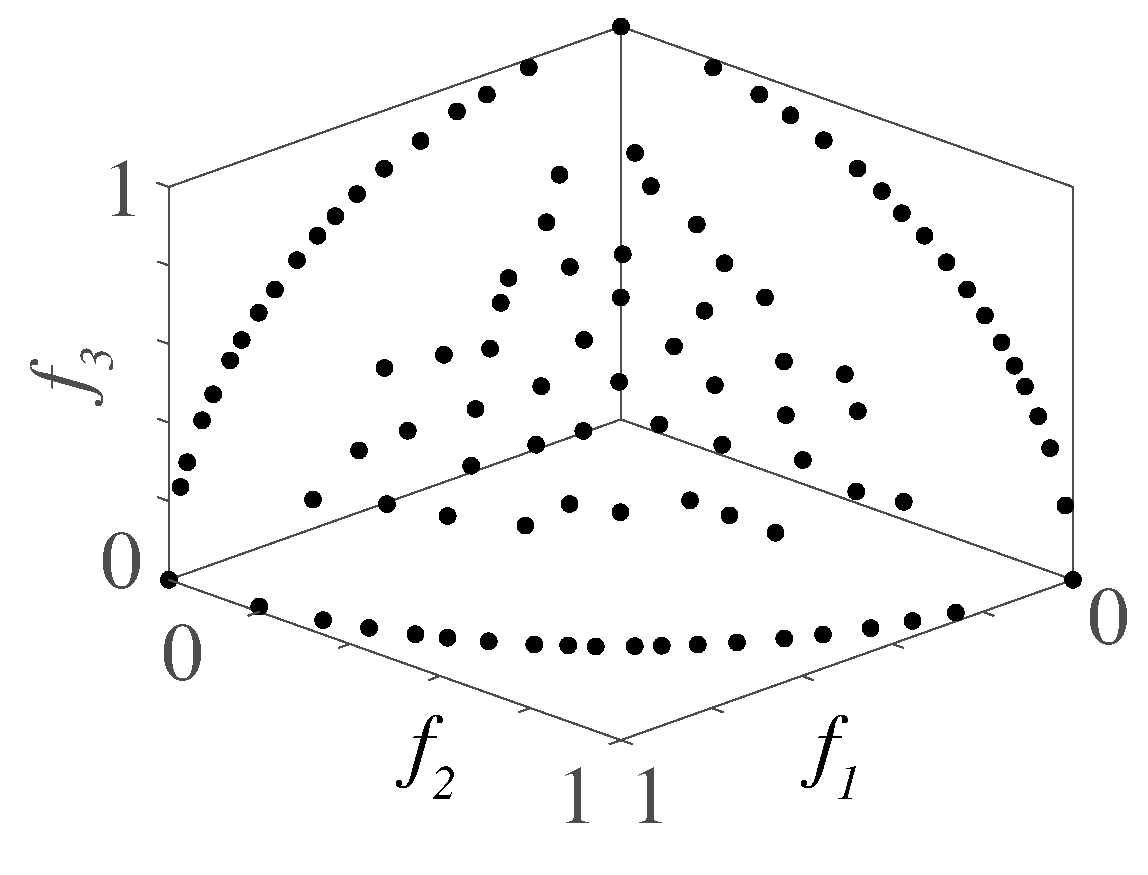
\includegraphics[width=1.5in]{FVEMOA_DTLZ4_3}}\quad
  \subfloat[FV-EMOA-LD]{\label{iudm1:b}
    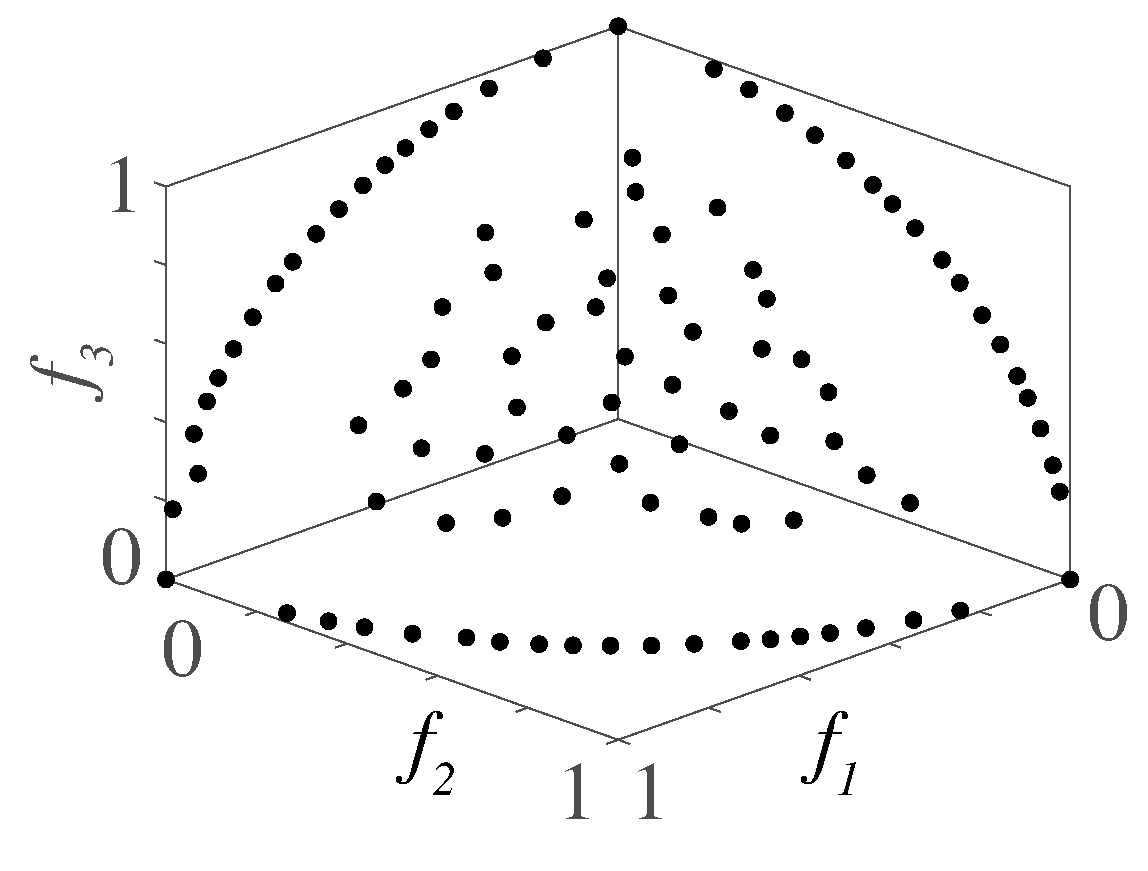
\includegraphics[width=1.5in]{FVEMOA_DR_DTLZ4_3}}\\
  \subfloat[FV-EMOA-CD]{\label{iudm1:c}
    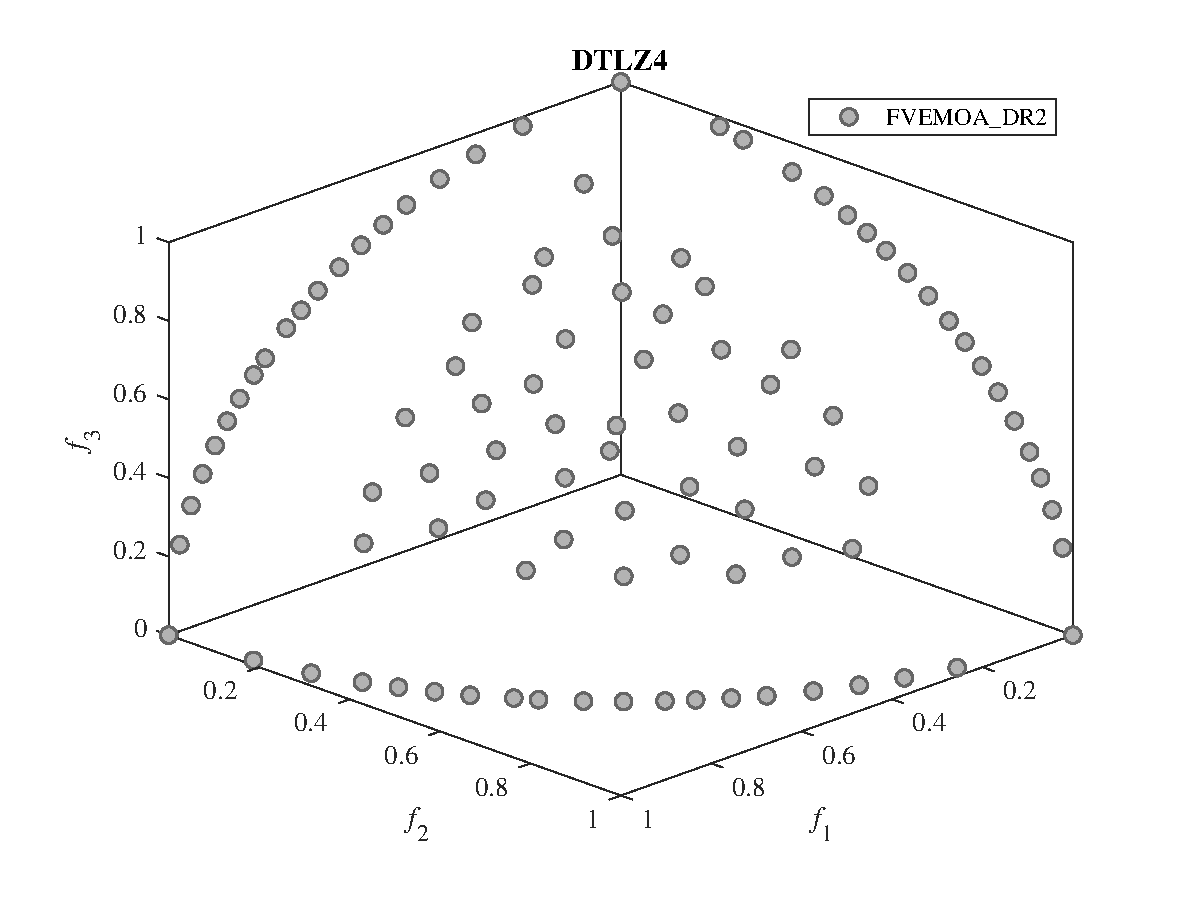
\includegraphics[width=1.5in]{FVEMOA_DR2_DTLZ4_3}}\quad
  \subfloat[FV-EMOA-Opt]{\label{iudm1:d}
    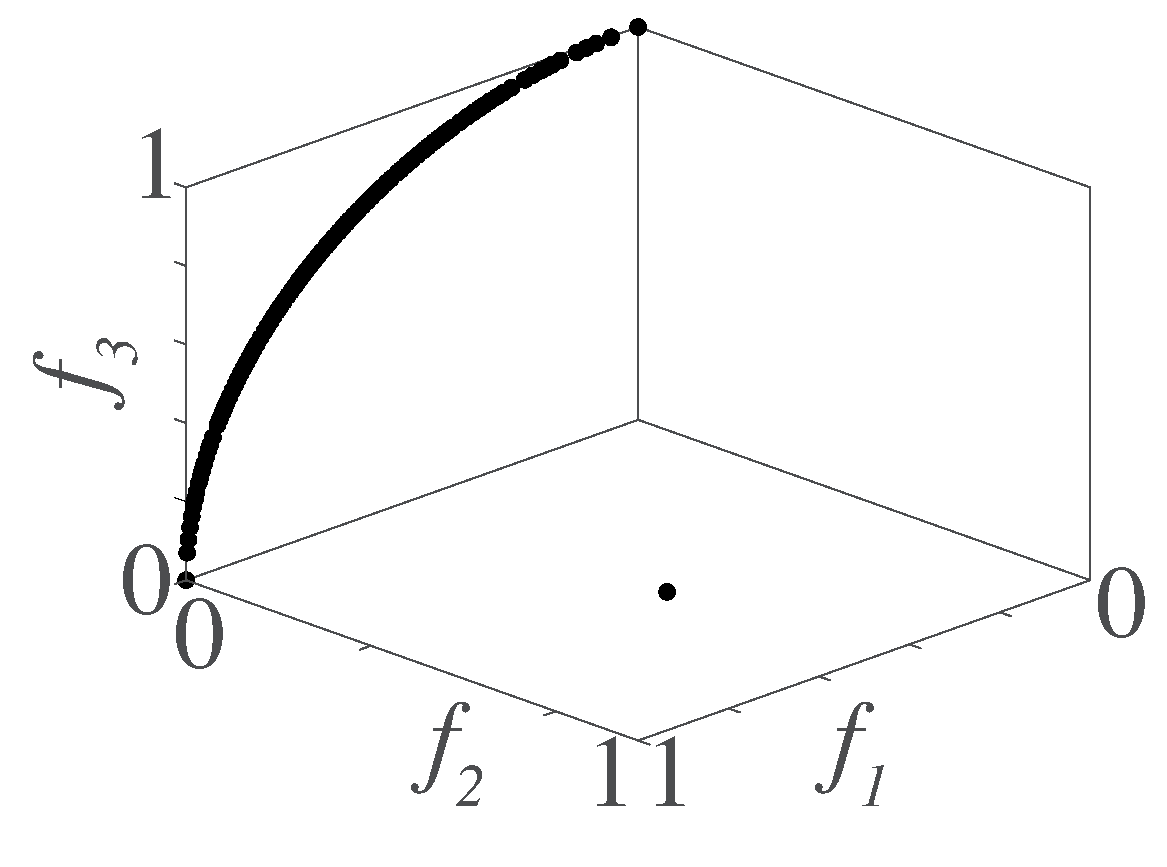
\includegraphics[width=1.5in]{FVEMOA_optimal_DTLZ4_3}}\\
  \caption{
    The final distribution of 4 reference point strategies on 3-dimensional DTLZ4 problems.
  }
  \label{iudm1}
\end{figure} 
\begin{figure}[!t]
  \centering
  \subfloat[FV-EMOA-2]{\label{iudm2:a}
    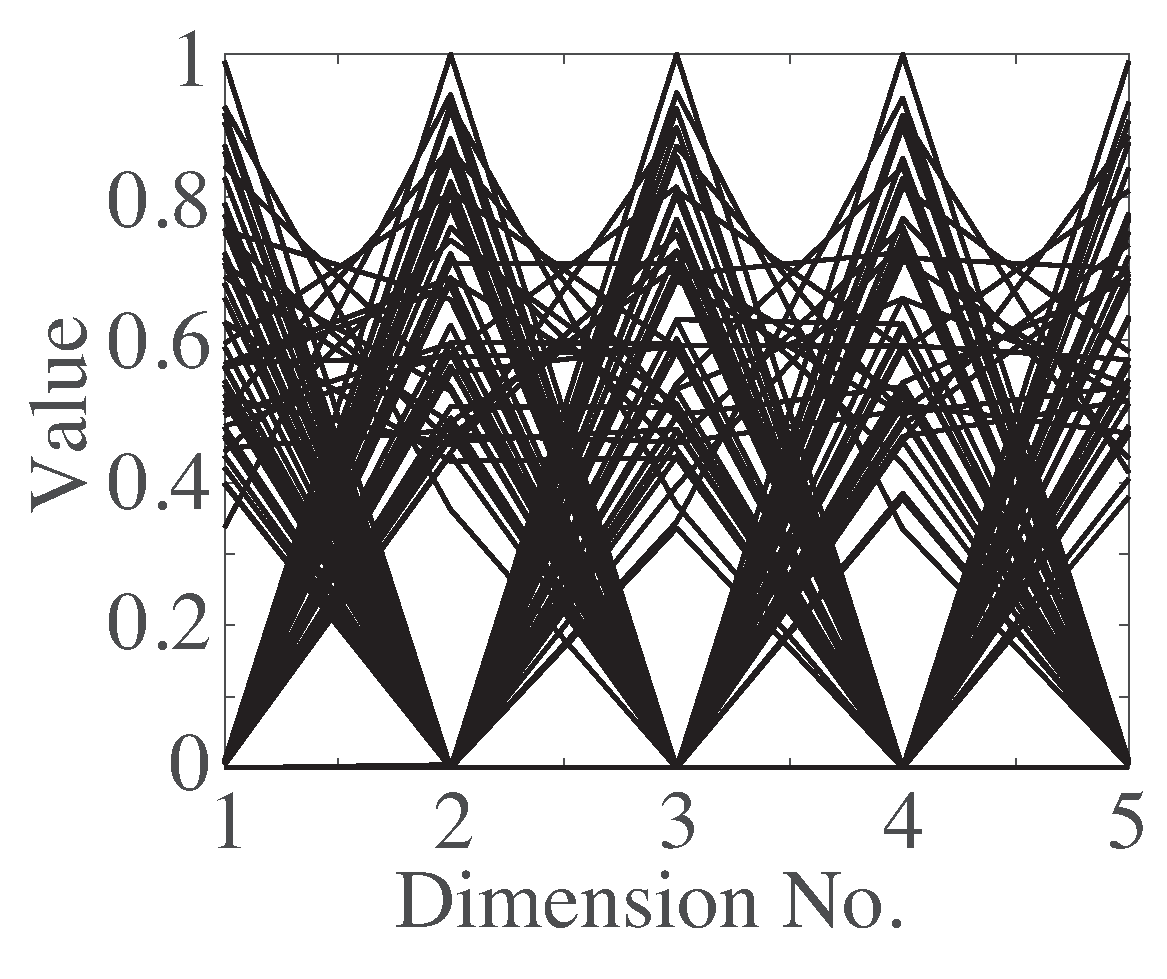
\includegraphics[width=1.5in]{FVEMOA_DTLZ4_5}}\quad
  \subfloat[FV-EMOA-LD]{\label{iudm2:b}
    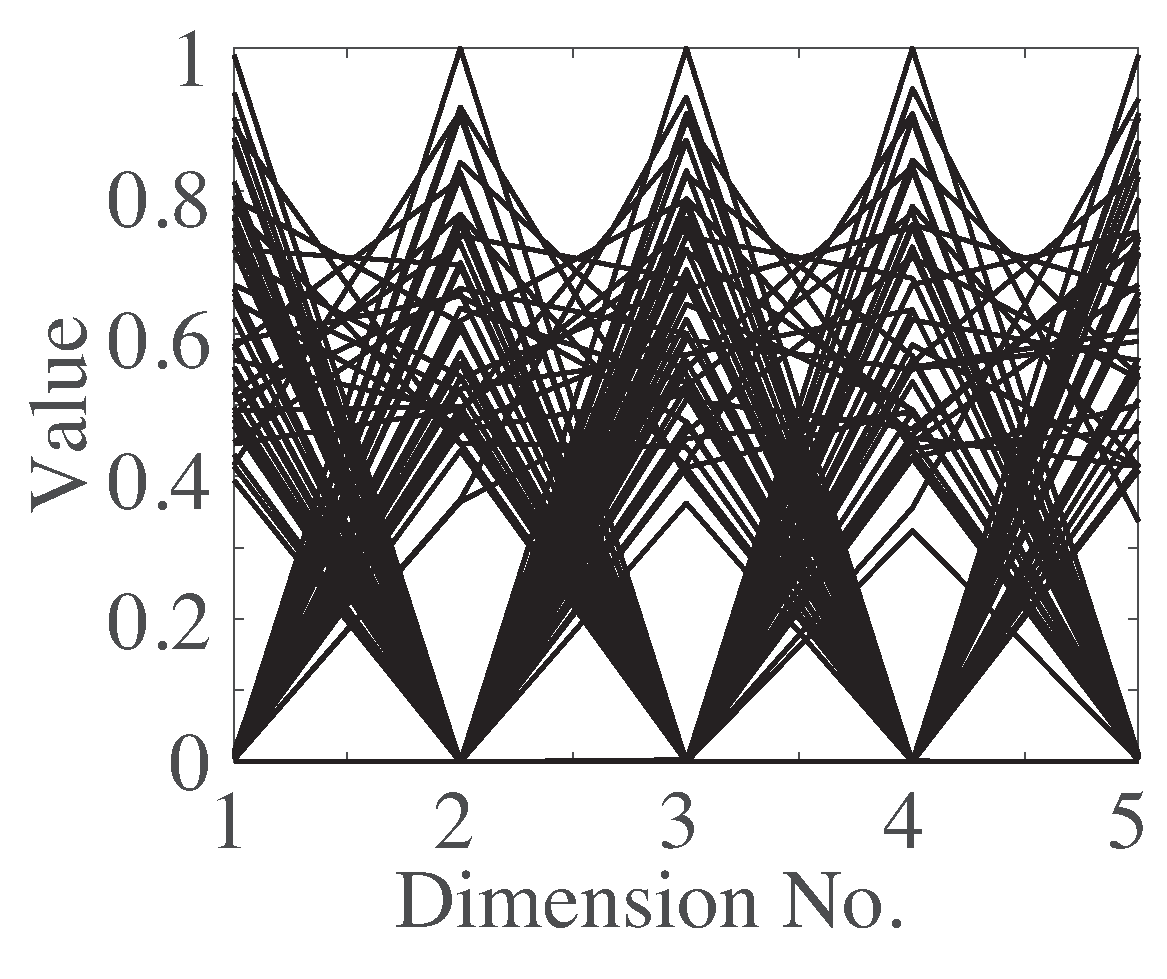
\includegraphics[width=1.5in]{FVEMOA_DR_DTLZ4_5}}\\
  \subfloat[FV-EMOA-CD]{\label{iudm2:c}
    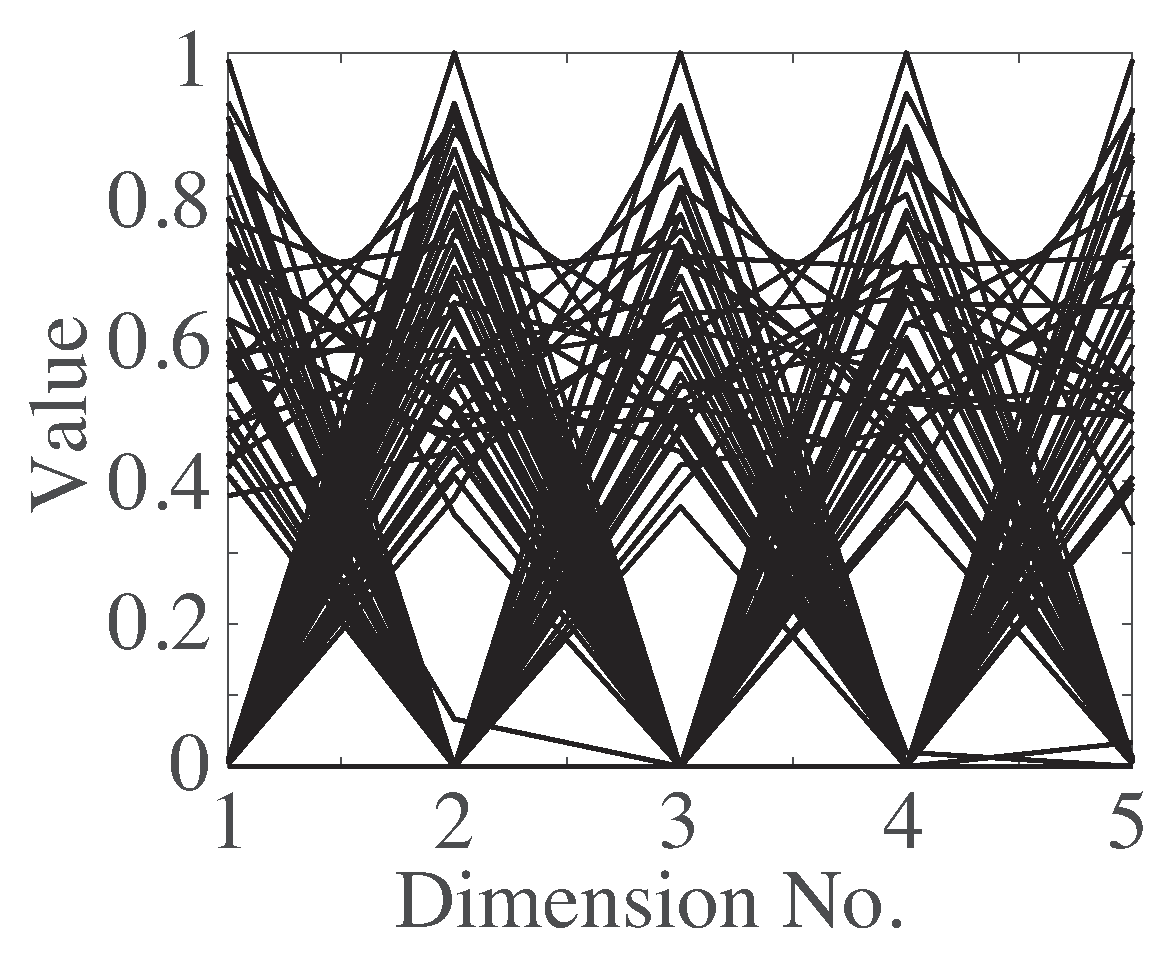
\includegraphics[width=1.5in]{FVEMOA_DR2_DTLZ4_5}}\quad
  \subfloat[FV-EMOA-Opt]{\label{iudm2:d}
    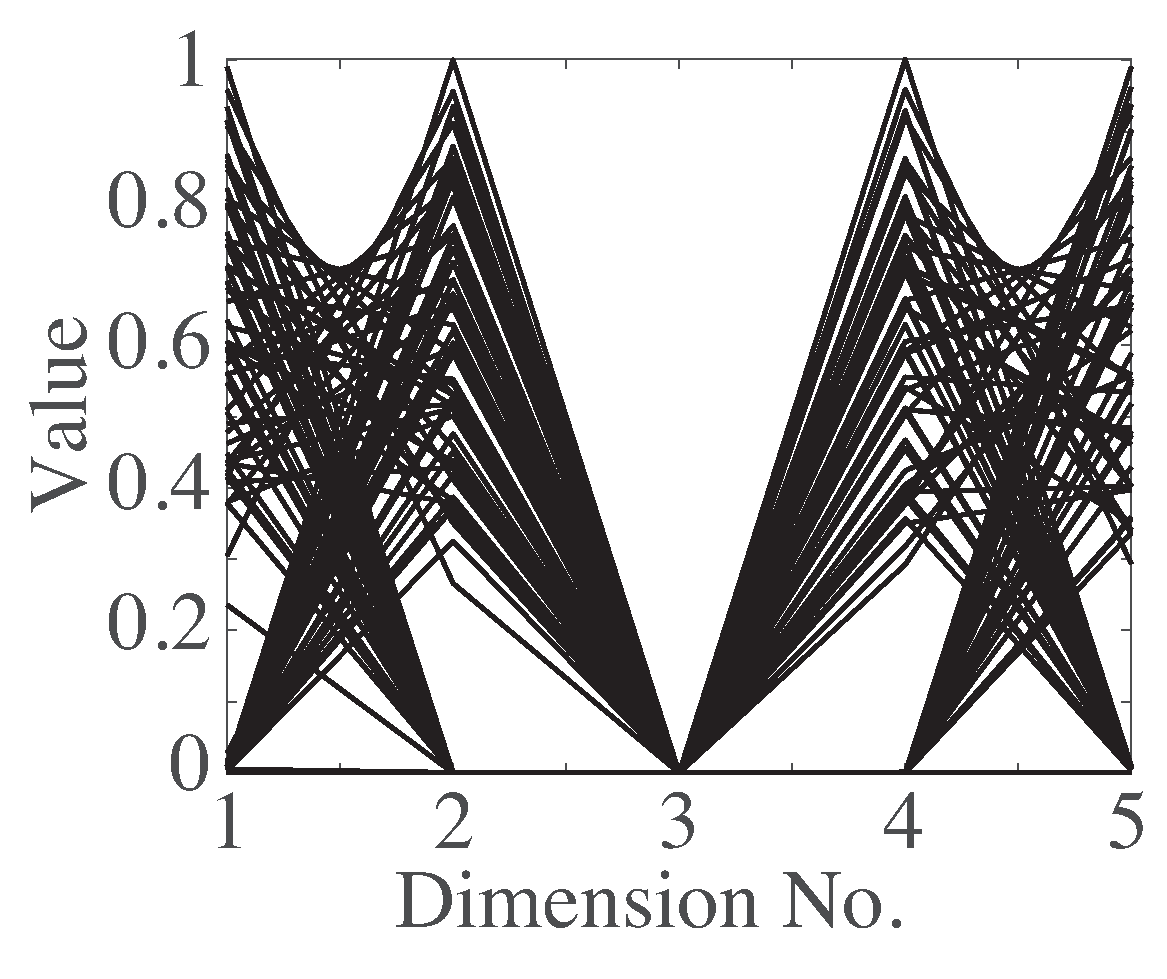
\includegraphics[width=1.5in]{FVEMOA_optimal_DTLZ4_5}}\\
  \caption{
    The final distribution of 4 reference point strategies on 5-dimensional DTLZ4 problems.
  }
  \label{iudm2}
\end{figure} 
The standard deviations of FV-EMOA-Opt on the DTLZ4 problem (shown in the TABLE \ref{table_FVEMOA_tri}) are both higher
than other three algorithms in 3- and 5-dimension($2.14e-1$  comparing with $1.21e-1, 1.31e-1, 1.76e-1$ in 3-dimension 
and $1.01e-1$ comparing with $9.98e-2, 7.21e-2, 6.05e-2$ in 5-dimension).
This observation also shows that the solutions distributions of some runs in FV-EMOA-Opt are poor over the total 20 runs.

In FV-EMOA-Opt, the algorithm applies $r_{Initial} = 1+1/H$ mechanism at the early stage of algorithm 
while other three algorithms apply $r_{Initial} = 2$.
Even though the $r_{final}$ of FV-EMOA-LD, FV-EMOA-CD and FV-EMOA-Opt are all equal to $1+1/H$, 
FV-EMOA-Opt can not jump out from the local minimum and estimate the pareto front well 
due to the pool searching behavior at the early stage. 

The above examples clearly show the importance of using dynamic mechanism, 
that a slightly larger $r$ than $1+1/H$ can make the algorithm with a better searching behavior in 
convergence stage where the solutions have not reached to the pareto front 
especially for the problems which are difficult to find the whole solutions space like the DTLZ4 problem. 

% ---------------sub-------------- Computational Experiments ------------------------------------
% ----------------------------- comparison of two dynamic mechanisms ----------------------------------
% 2种机制比较
% 当evaluation足够的时候,差不多
% feasible region 大, evaluation不太够时但过了convergence点时 我的好
% rinit = 10
%
\subsection{Comparison of Two Dynamic Mechanisms}
We want to further investigate the differences between two dynamic mechanisms 
(the linearly decrease mechanism and the weak convergence detection mechanism). 
Here are the examples of the final distribution on the MaF1 problem(as shown in Fig. \ref{ctdm}).
The total evaluation number is set to $3500$ and the convergence is detected at $3400$ evaluations. 
The solutions distribution of FV-EMOA-CD(Fig. \ref{ctdm:c}) is similar to 
the that of FV-EMOA-Opt(Fig. \ref{ctdm:d})
while there are still overmany solutions at the boundary of pareto front in FV-EMOA-LD(Fig. \ref{ctdm:b}). 

The reason is quite intuitionistic.
In the linearly decrease mechanism, the total evaluation number is so small that it is too late for the solutions 
to distribute evenly when reaching to the final generation. 
But in the weak convergence detection mechanism, a convergence is reported after 3400 evaluations and 
the algorithm still has 100 evaluations to make a good solutions distribution. 
% conclusion里写
\begin{figure}[!t]
  \centering
  \subfloat[FV-EMOA-2]{\label{ctdm:a}
    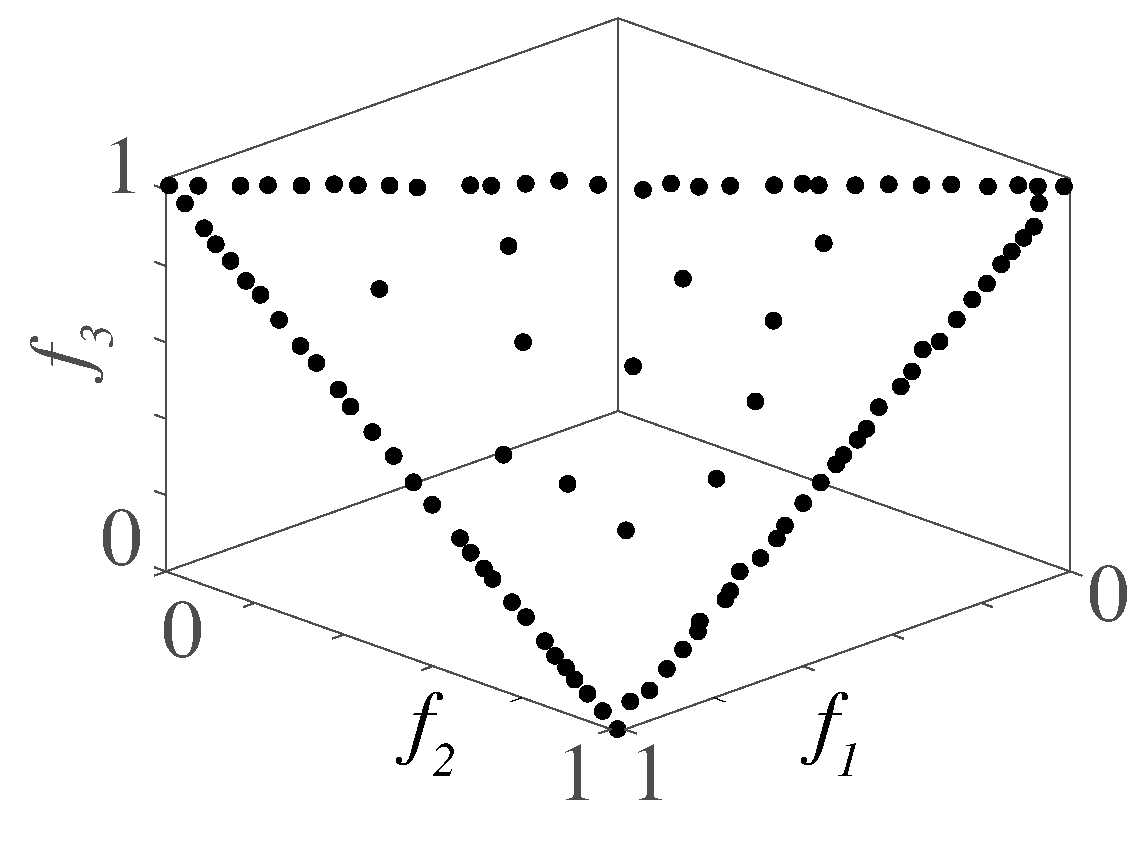
\includegraphics[width=1.5in]{FVEMOA_MaF1_M3_3500_3400convergence}}\quad
  \subfloat[FV-EMOA-LD]{\label{ctdm:b}
    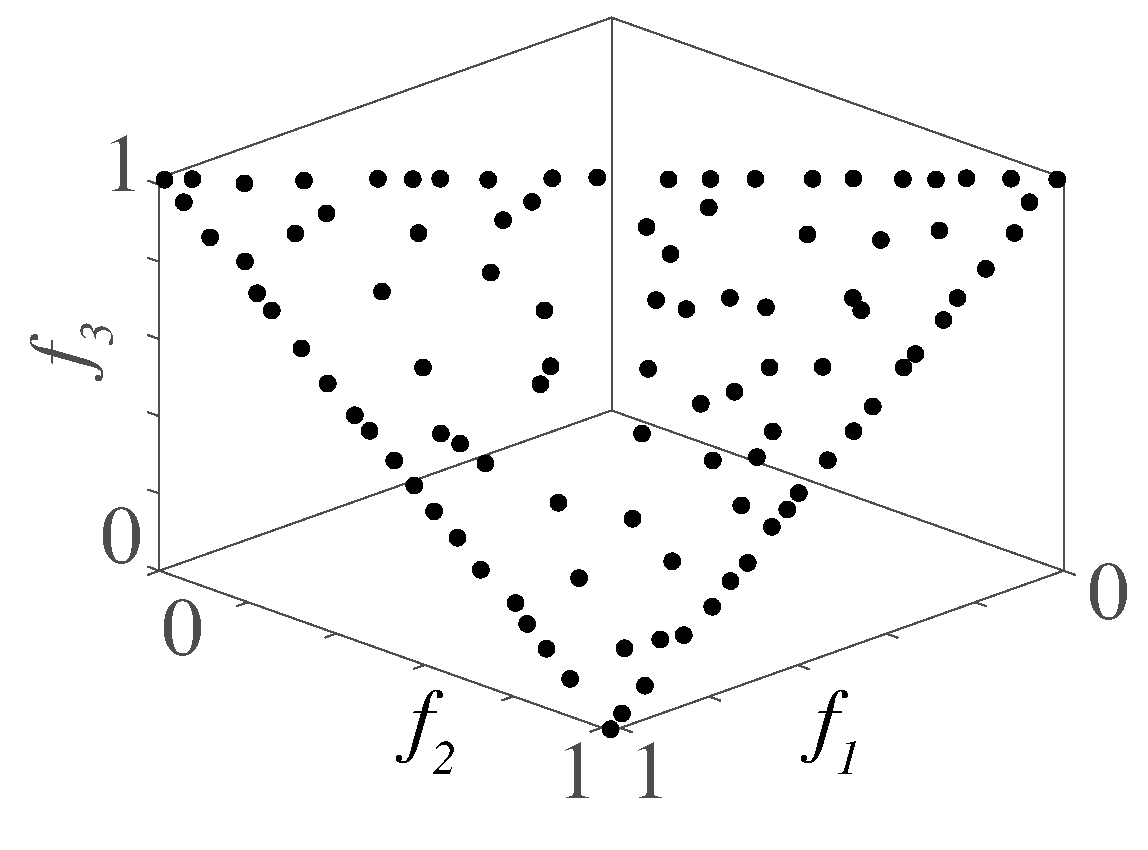
\includegraphics[width=1.5in]{FVEMOA_DR_MaF1_M3_3500_3400convergence}}\\
  \subfloat[FV-EMOA-CD]{\label{ctdm:c}
    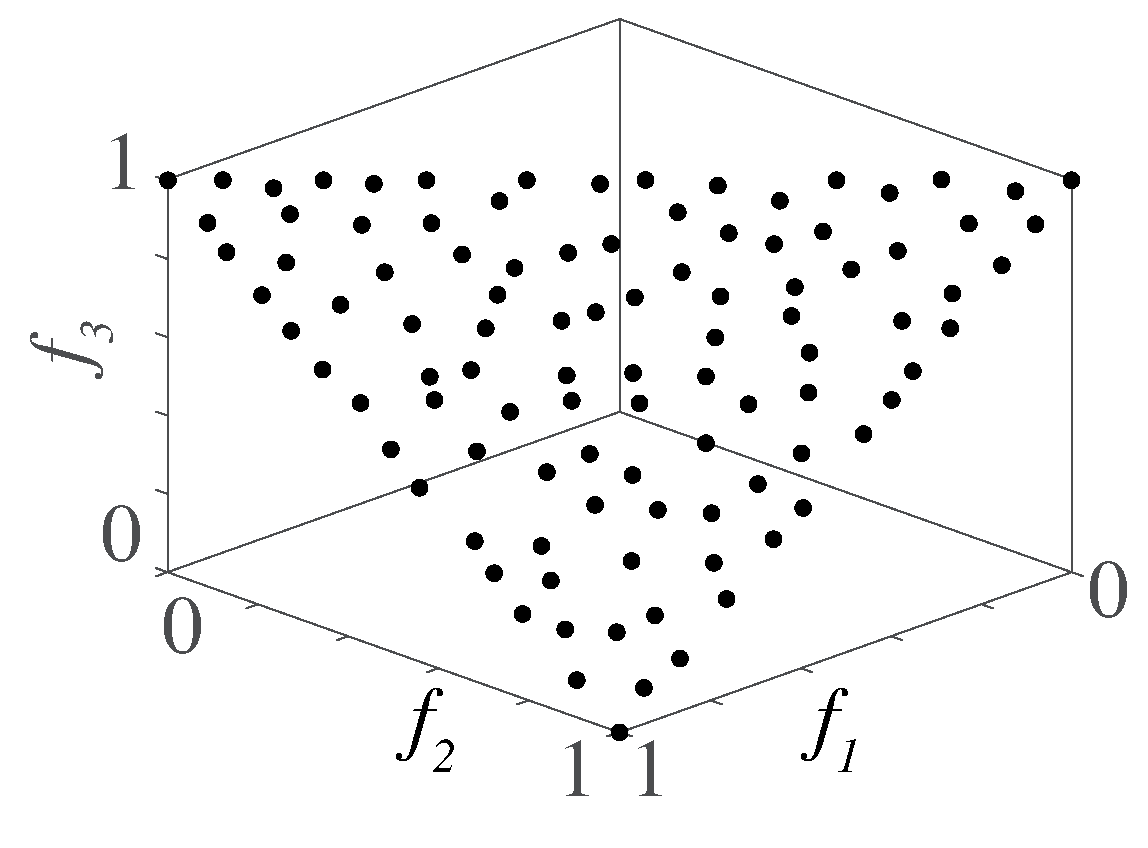
\includegraphics[width=1.5in]{FVEMOA_DR2_MaF1_M3_3500_3400convergence}}\quad
  \subfloat[FV-EMOA-Opt]{\label{ctdm:d}
    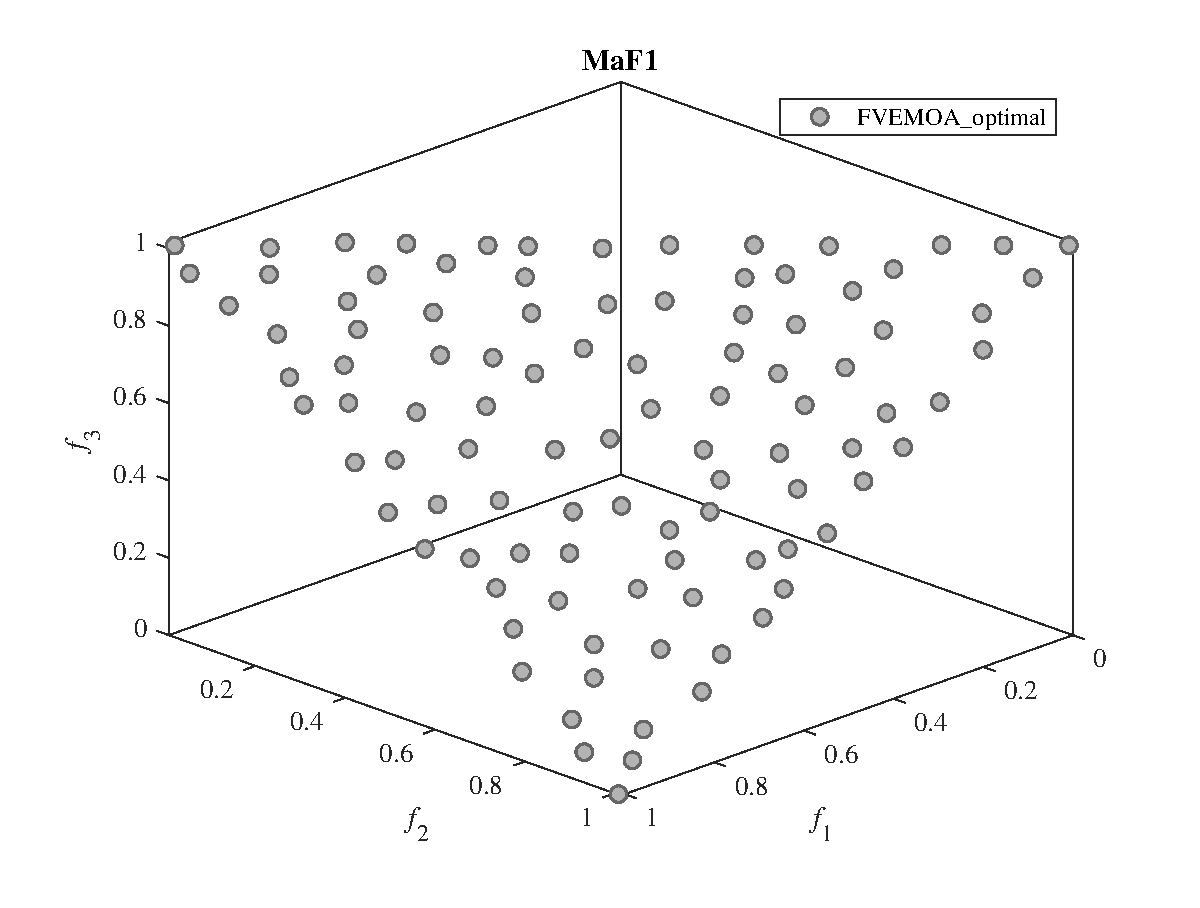
\includegraphics[width=1.5in]{FVEMOA_optimal_MaF1_M3_3500_3400convergence}}\\
  \caption{
    The final distribution of 4 reference point strategies on the MaF1 problem.
    The results are obtained after $3500$ evaluations($t_{Convergent} = 3400$).
  }
  \label{ctdm}
\end{figure} 

\section{Conclusions}
In this paper, we emphasize the importance of reference point adaptation 
in indicator-based EMOA by a simple example. 
% Without a reference point adaptation mechanism, the diversity of the final solutions will be poor
% on inverted-shape pareto front problems. 
% This phenomenon will not be observed on the triangular pareto front problems. 
Then we state the dynamic reference point adaptation mechanism with the illustration by two aspects:
\subsubsection{Optimal Distribution} Considering the flat triangular problems, 
the optimal setting of hypervolume reference point is $r=1+1/H$. 
\subsubsection{Better Searching Behavior} In the early stage, 
the solutions may not be close to the true pareto front. 
A slightly larger value of $r$ can achieve a better searching behavior 
especially on the problems which are difficult to find the whole objective space. 
We give an example of the DTLZ4 problem. 

After that, a new dynamic reference point adaptation mechanism is proposed in this paper.
A weak convergence detection mechanism is used. 
We apply our new dynamic mechanism on many test problems containing triangular, inverted-triangular pareto fronts problems.
The results show that FV-EMOA with $r=2$ performs the worst on the problems with inverted-triangular pareto fronts. 
FV-EMOA with weak convergence detection mechanism performs better or worse than FV-EMOA with linearly decrease mechanism
but performs no significant difference comparing with FV-EMOA when $r=1+1/H$.

We compare our new mechanism with the proposed linearly decrease mechanism and find that
on some conditions, specifically the condition that the total evaluation number 
is limited to a small addition after the reported convergence, 
our weak convergence detection mechanism performs better than linear decrease mechanism
especially on the problems with the small feasible region and easy mapping from decision space to objective space. 

In the future, we plan to further investigate the behavior of our new mechanism. 
A larger dimensionality of MaOPs should be considered 
and the problems with different pareto front shapes should be tested and analyzed detailedly. 
Our weak convergence detection mechanism can also be further improved.

\bibliographystyle{IEEEtran} 
\bibliography{mybibtex} 

\end{document}


